%%%%%%%%%%%%%%%%%%%%%%%%%%%%%%%%%%%%%%%%%
% Arsclassica Article
% LaTeX Template
% Version 1.1 (10/6/14)
%
% This template has been downloaded from:
% http://www.LaTeXTemplates.com
%
% Original author:
% Lorenzo Pantieri (http://www.lorenzopantieri.net) with extensive modifications by:
% Vel (vel@latextemplates.com)
% Johan Bos (johan.bos@rug.nl)
%
% License:
% CC BY-NC-SA 3.0 (http://creativecommons.org/licenses/by-nc-sa/3.0/)
%
%%%%%%%%%%%%%%%%%%%%%%%%%%%%%%%%%%%%%%%%%

%----------------------------------------------------------------------------------------
%	PACKAGES AND OTHER DOCUMENT CONFIGURATIONS
%----------------------------------------------------------------------------------------

\documentclass[
10pt, % Main document font size
a4paper, % Paper type, use 'letterpaper' for US Letter paper
oneside, % One page layout (no page indentation)
%twoside, % Two page layout (page indentation for binding and different headers)
headinclude,footinclude, % Extra spacing for the header and footer
%BCOR5mm, % Binding correction
] {book}% {scrartcl}

\input{structure.tex} % Include the structure.tex file which specified the document structure and layout


%----------------------------------------------------------------------------------------
%	HYPHENATION
%----------------------------------------------------------------------------------------
% Specify custom hyphenation points for particular words with dashes where
% hyphenation is allowed, or alternatively, don't put any dashes in a
% word to prevent hyphenation altogether. Expand this list as needed.
\hyphenation{Fortran hy-phen-ation}



%----------------------------------------------------------------------------------------
%	TITLE AND AUTHOR(S)
%----------------------------------------------------------------------------------------

\title{\normalfont\spacedallcaps{title}} % The article title

\author{\spacedlowsmallcaps{author}} % The article author(s) - author affiliations need to be specified in the AUTHOR AFFILIATIONS block

\date{} % An optional date to appear under the author(s)

%----------------------------------------------------------------------------------------

\begin{document}

%----------------------------------------------------------------------------------------
%	HEADERS
%----------------------------------------------------------------------------------------

%\renewcommand{\chaptermark}[1]{\markright{\spacedlowsmallcaps{#1}}} % The header for all pages (oneside) or for even pages (twoside)
%\renewcommand{\subsectionmark}[1]{\markright{\thesubsection~#1}} % Uncomment when using the twoside option - this modifies the header on odd pages
%\lehead{\mbox{\llap{\small\thepage\kern1em\color{halfgray} \vline}\color{halfgray}\hspace{0.5em}\rightmark\hfil}} % The header style

\pagestyle{scrheadings} % Enable the headers specified in this block


%----------------------------------------------------------------------------------------
%	TITLE PAGE
%----------------------------------------------------------------------------------------

\hypersetup{pageanchor=false}
\begin{titlepage}
\thispagestyle{empty}
\begin{figure}[h!] %  figure placement: here, top, bottom, or page

\includegraphics[width=4in]{ruglogo} 
% 
\includegraphics[width=4in]{ruglogo-nl}   % Dutch version
\end{figure}

\begin{center}
\vspace{30 mm}
\begingroup \linespread{1,75} \selectfont 
\textsc{\LARGE Comparing Human and LLM Annotation of Media Frames in the ChangeMyView Dataset}\\
\endgroup

Anya Kiewit\\[2.5cm]

\end{center}
\vfill
\textbf{Bachelor Thesis}\\  
Informatiekunde\\  %Information Science\\
Anya Kiewit\\
S5168767\\
\today
\end{titlepage}
\hypersetup{pageanchor=true}



%----------------------------------------------------------------------------------------
%	ABSTRACT
%----------------------------------------------------------------------------------------

\pagenumbering{roman}
\chapter*{Abstract}
\markboth{Abstract}{Abstract}
\addcontentsline{toc}{chapter}{Abstract}
Although Large Language Models (LLMs) are highly efficient at processing structured formal data, their ability to interpret informal human communication remains a major challenge. Understanding this limitation is crucial if we want to use LLMs to speed up the analysis of online discussions. In current research, there are two big gaps. First, most research that tests models on framing tasks uses formal text as datasets, making it unclear how well LLMs handle finding frames in informal and persuasive discussions, like those on the ChangeMyView (CMV) subreddit. Second, while studies show that AI advice can bias human annotators on factual datasets, they miss what happens when humans get LLM suggestions for subjective tasks. This is crucial to see whether humans become overly dependent on LLM suggestions, which affects maintaining the quality and reliability of the dataset.

This research fills these gaps by testing both stand-alone models and hybrid human-LLM teams on the CMV dataset. To do this, a dataset of 495 unique comments was sampled from CMV. A human gold standard was created using \citeauthor{card2015media}'s \citeyearpar{card2015media} 15 framing dimensions. Different models were tested, to see how well they can perform the task. Finally, a user study looked at how humans and LLMs work together. It compared how humans annotate on their own against how they perform when they get LLM suggestions, allowing us to measure automation bias.

Our results show that while humans remain highly effective at interpreting implicit meaning, LLMs consistently struggle with these nuances. Furthermore, the hybrid annotation workflow failed to improve performance. Instead, it led to automation bias, which caused f1-scores to drop whenever participants accepted wrong LLM suggestions. This study concludes that without critical human oversight, current human-LLM collaboration can actually lower the quality instead of improving it. Because of this, human annotators are still necessary for framing tasks, and hybrid workflows need to be set up in a way that encourages annotators to stay critical of the LLM suggestions.




%----------------------------------------------------------------------------------------
%	TABLE OF CONTENTS & LISTS OF FIGURES AND TABLES
%----------------------------------------------------------------------------------------
\clearpage
\setcounter{tocdepth}{3} % Set the depth of the table of contents to show sections and subsections only
\tableofcontents % Print the table of contents

%\listoffigures % Print the list of figures (optional, only if you have many figures)

%\listoftables % Print the list of tables (optional, only if you have many tables)

%\lstlistoflistings



%----------------------------------------------------------------------------------------
%	Preface
%----------------------------------------------------------------------------------------

\chapter*{Preface}
\markboth{Preface}{Preface}
\addcontentsline{toc}{chapter}{Preface}

After months of annotation, model training and writing, this thesis is now finished. I wrote this thesis as part of the bachelor program Information Science at the University of Groningen. During my studies, I have seen that LLMs have become much better at different tasks, for example, answering more complex questions. Because of the subjectivity of the task, I was excited to test whether LLMs were already better at the framing task than humans. Beforehand, I expected that the models would do a better job at the task than they actually did. It shows that there is still a lot of room for improvement when it comes to framing tasks.
When looking at the final results, I noticed something else that I became curious about. I thought the participants in the experiment would follow the LLMs suggestions even more. I am curious why that is, whether they think that they are better at the task than LLMS, or they just simply do not trust LLMs. This is definitely something to investigate further in future research, especially since it connects information science with fields like psychology.

I want to thank my thesis supervisor, Khalid Al-Khatib, for providing us with the dataset and giving relevant feedback. I also want to thank Floris and Julius, for the annotating, so we could create the gold standard as a group. Although the task was quite time consuming, I am happy that we pushed through and managed to achieve the results we have. 

%----------------------------------------------------------------------------------------
%	INTRODUCTION
%----------------------------------------------------------------------------------------

\chapter{Introduction}
\pagenumbering{arabic}
In the last couple of years, the use of Large Language Models (LLMs), such as ChatGPT, has increased rapidly. There have been concerns about the reliability of the generated texts, and an increasing number of studies have been done researching the potential of using LLMs as members of hybrid teams \citep{richter2024hybrid}. Despite their growing popularity, it remains unclear to what extent LLMs improve the quality and reliability of human work. \cite{wilkens2020artificial} states that AI tends to be a more valuable tool in situations where continuous monitoring and information processing are needed, but it has shortcomings in fields with a high need for creative problem solving and communication to build trust. 

Although LLMs demonstrate high efficiency in processing structured formal data, their ability to interpret informal human communication remains the subject of debate \citep{wilkens2020artificial}. Informal discussions often rely on implicit meanings and creative language use, which continue to present challenges for automated systems. Identifying "frames", defined as the specific perspectives used to present an argument, such as 'Economic' or 'Political' perspectives, requires a deep understanding of nuance, cultural context, and communicative intent \citep{card2015media}. For example, while the isolated word "money" might typically be labelled under 'Economic', its context within a full sentence alters the appropriate framing. In the sentence, "Giving people financial aid after a disaster helps them live a happier life," the correct frame shifts to 'Quality of Life'. Because of this, humans may still maintain an advantage over LLMs in frame annotation tasks. Understanding this distinction is important for evaluating whether LLMs can function reliably as stand-alone tools or whether they are more effective when used collaboratively with humans. 

To investigate the issue of LLMs limitations in understanding nuanced human communication, the ChangeMyView (CMV) subreddit provides a suitable dataset.  CMV is an online platform where Reddit users can start a discussion with a specific opinion and other user can give arguments against this opinion to prove the original post is untrue. CMV consists of highly persuasive, informal, and often emotionally charged discussions, in addition, the quality is being checked by moderators \citep{tan2016winning}. These characteristics make the dataset particularly valuable for studying the ability of both humans and LLMs to identify frames in complex online discussions. 

Understanding how LLMs handle framing is important for several reasons. First, annotation tasks are very time consuming. Shortening the time it takes to annotate means that there is more data available for researchers to analyse large amounts of online debates. Second, it can tell us whether humans become overly dependent on using LLM suggestions when performing the task. This is crucial to maintaining the quality and reliability of the dataset. To explore this further, human-LLM collaboration can work in two main ways, LLMs can do tasks completely on their own without any human help, or they can work together in a hybrid team. The next chapter will explain these different setups of human-LLM interaction.


This study examines the performance of humans and LLMs in the frame annotation task of the CMV dataset. In addition, this study investigates the influence of human-LLM collaboration on annotation performance. More specifically, it explores whether human annotators critically evaluate LLM suggestions or become biased toward accepting them.

\newpage

This study seeks to answer the following research question:\\ 
    \textit{“How accurate are LLMs compared to humans for the frame annotation task of the ChangeMyView dataset and what is the influence of humans and LLMs working together on the annotation task?”}\\




Leading to the following sub-questions:
\begin{enumerate}
    \item \textit{``How accurate are humans in the frame annotation task of the ChangeMyView dataset?''}
    \item \textit{``How accurate are LLMs in the frame annotation task of the ChangeMyView dataset?''}
    \item \textit{``How do the results of the LLMs compare to the human results?''} 
    \item \textit{``What is the influence of humans and LLMs working together on the results of the frame annotation task of the ChangeMyView dataset?''}
\end{enumerate}


Our results show a massive gap between the models and humans, with even ChatGPT-4o falling heavily short of the human baseline. Also, while LLM suggestions made human annotators agree with each other more, it actually lowered their overall score because they often agreed on the wrong frames by copying the LLMs mistakes.

The remainder of this thesis is structured as follows. Chapter 2 presents the relevant background literature. Chapter 3 covers the collection of the dataset, the annotation tasks, answering sub-question 1, and the processing steps used. Chapter 4 describes the methods used to answer the rest of the sub-questions, while Chapter 5 details the results and discussion. Lastly, Chapter 6 provides the conclusion and outlines the limitations of this study.




\chapter{Background}
To understand how humans and LLMs handle framing on CMV, we need to look at two main areas. First, we need to look at hybrid annotation workflows, focussing on how LLMs compare to humans and how working together affects data quality. Second, we look at media framing and why informal, emotional language on platforms like CMV makes framing so difficult. Together, these sections show what we already know and point out the gaps that this study aims to fill.

\section{Hybrid annotation workflows}
As LLMs are increasingly integrated in tasks that involve reasoning, classification, and text interpretation, more research has been conducted on their impact. For example, \cite{belcavello2025evaluating} evaluates the impact of semi-automating FrameNet semantic annotation by comparing manual human effort, fully automatic machine results, and a hybrid "Machine plus Human" approach. They found that hybrid annotation increases frame diversity and maintains similar coverage to human-only settings while preserving interpretive depth. Although fully automatic annotation performed significantly worse across most metrics and the hybrid model only slightly reduced overall annotation time, the semi-automatic workflow was shown to be a sustainable method for large-scale dataset growth. 

Highlighting the performance gap between general-purpose LLMs and task-specific models, \cite{boitel2023comparative} found that task-specific BERT architecture (DeBERTa-v3-Large) achieved a 95\% accuracy for emotion recognition on the BAUM dataset compared to GPT-3.5's (Davinci) 82.8\%. Although GPT-3.5 showed higher throughput and handled data imbalances better, BERT's specialized architecture still achieved a higher accuracy. Although the authors note that models like GPT-4 may narrow this gap, these current limitations show that stand-alone LLMs still struggle with complex, subjective text. That is why researchers still need hybrid, human-in-the-loop workflows.

A similar conclusion was found by \cite{kunjar2025computational} when looking specifically at framing tasks. They tested LLMs on news coverage and found that while these LLMs are helpful they are still often outperformed by manual human coders or smaller, specialized model. This shows again that stand-alone LLMs struggle with complex tasks like finding frames, and proves why we still need humans or hybrid teams to get the best results.

Despite its advantages in scalability, hybrid annotation may have unintended consequences for annotator behaviour and data quality. While \cite{belcavello2025evaluating} argue that hybrid annotation is a sustainable method for large-scale dataset growth, \cite{schroeder2025just} warn of the psychological and systematic effects of this approach on the human annotator. The researchers conclude that providing LLM-generated suggestions for subjective annotation tasks does not reduce the time spent on the task, but does significantly increase annotators' self-reported confidence and task understanding. Furthermore, they found that annotators strongly adopt these AI suggestions, which homogenizes the "ground truth" toward the LLMs baseline and significantly alters the label distribution compared to unassisted human work.

\cite{beck2026bias} investigate the psychological factors and system designs that influence human performance during the dependent verification of AI-generated pre-annotations. Tasking 2,784 participants with auditing greenhouse gas emissions data, the researchers analysed how interface design and user disposition affect the tendency toward under-correction. The experiment proved that human-AI loops are highly vulnerable to automation bias when interfaces require higher physical workload to overwrite errors. Furthermore, while financial incentives and early experiences with AI accuracy failed to alter human behaviour, individual attitudes toward automation and the conceptual complexity of the data were the definitive factors shaping whether humans successfully corrected or adopted to flawed AI recommendations.

To optimize the trade-off between annotation speed and data quality, \cite{wang2024human} proposed the LAPRAS framework. This collaborative framework enhances text annotation efficiency by combining machine-generated labels with strategic human verification. In this multi-step process, LLMs generate both labels and natural language explanations, which a separate verifier model then assesses to identify a subset of potentially incorrect annotations for human review.
Experimental results across several benchmarks show that this method can improve overall dataset accuracy by at least 10\% while requiring humans to re-annotate only 15\% of the data. While human-subject studies showed smaller but still substantial gains around 7-8\%. Further human studies indicate that while LLM-generated explanations assist in understanding decisions, their effectiveness in the re-annotation phase depends significantly on their quality and the specific task context.

\section{Media framing on social platforms}
An important question is whether these performance differences extend in other annotation tasks, such as the categorization of media frames. \cite{card2015media} introduces the 15 framing dimensions that we will use in this research. They define framing as the specific aspect of a topic that an argument emphasizes. The same topic can be discussed from different angles. The chosen angle is the frame, and it influences how audiences interpret the message.

This challenge is further amplified by the nature of the text being analysed. While previous research has been done on reliable and formal text. \cite{belcavello2025evaluating}, for example, used sentences from a corpus of television news media in Brazilian Portuguese. On the other hand, the CMV Reddit page is a page where people want to have discussions and maybe change their view on a specific topics. A foundational study by \cite{tan2016winning} shows that persuasion on this platform relies heavily on the back-and-forth conversation and the words people choose. Most people do not use formal language in their comments and write their own unfiltered opinions. This makes the data highly emotional in nature, domains where, as \cite{wilkens2020artificial} notes, AI tools often show shortcomings due to a lack of emotional reflection and social intelligence. 


\section{Research gap}
There are two big gaps in the current research. First, most paper that test models on framing tasks use formal news media as dataset \citep{belcavello2025evaluating, kunjar2025computational}. It is still unclear how well LLMs handle finding frames in informal and persuasive discussions, like those on the CMV subreddit. Second, while studies show that AI advice can bias human annotators \citep{schroeder2025just, beck2026bias}, they mostly look at factual datasets, and miss what happens when humans get LLM suggestions for emotional and subjective tasks. This research fills these gaps by testing both models and human-LLM teams on the CMV dataset.

\chapter{Data and Material}
This chapter describes the collection of the dataset, the annotation, and processing steps used in this study. It begins by explaining the data collection process, including the source dataset from the ChangeMyView (CMV) subreddit and the strategy used for comment selection and sampling. Next, it introduces the annotation framework, including the 15 frame definitions, the labeling guidelines, the tool used for this task, and the inter-annotator agreement. Then Finally, this chapter outlines the processing pipeline, including data cleaning, gold standard construction, and prompt engineering for the LLM. 

\section{Collection} 
This section explains the data collection process, including the source dataset from the CMV subreddit, as well as the strategy used for the comment selection and sampling. Together, these steps outline how the dataset of 500 comments were gathered before moving into the annotation phase.

\subsection{Source dataset}
\label{sec:CMV}
The online discussions came from the sub-Reddit page ChangeMyView (CMV)\footnote{\url{https://www.reddit.com/r/changemyview/}}. The thesis supervisor provided us with a dataset with all the discussions and their meta data from the year 2005 to 2017, the Webis-CMV-20 dataset\footnote{\url{https://zenodo.org/records/3778298}}. For this research, only the discussions are used and none of the meta data.  From this dataset the thesis supervisor provided us with a sub-set of 50 discussions from the Webis-CMV-20 dataset. To make sure this data is high quality and covers different topics, these threads were filtered on comment richness, post completeness, topic uniqueness, and a balance across the years 2013 to 2017. All the specific specific sampling filters, engagement metrics, and structured statistics are in Appendix \ref{sec:dataset_stats}. 

Regarding the structure, each discussion consists of an 'Original Post (OP)', the post that started the discussion. Each OP has people reacting on it, these are the comments. For example, one OP can have one comment or can have over 50 comments. 

\subsection{Comment selection and sampling}
Out of these 50 discussions a sub-set of 500 comments had to be chosen to use as final dataset, as requested by our thesis supervisor. For the first 200 comments, a sample from a parallel student research project was used because of an opportunity to compare the different annotations in future research. 

To expand this dataset to a total of 500 comments, another 300 comments needed to be selected from the remaining data within the same 50 discussions. Instead of choosing these 300 comments manually, an LLM was used to randomly sample them. Using an LLM was the best option for two reasons. First, letting a human pick the comments takes more time and introduces selection bias because humans might unconsciously pick shorter or simpler comments. Using an LLM ensures a completely randomized and unbiased selection from the remaining threads. Second, the LLM could write and execute the data selection code very quickly. The prompt used to select the last 300 comments can be found in Appendix \ref{sec:sampling_prompt}.




\section{Annotation}
This section describes the set of 15 argumentative frames used to capture different perspectives, as well as the labeling guidelines applied during annotation. These guidelines define how frames should be identified and how multiple frames within a single comment are handled. Together, the framework and guidelines ensure a consistent and structured approach to assigning labels across the dataset. Label Studio \footnote{\url{https://labelstud.io/}}, an open-source annotation tool, is used to organize and annotate the dataset. Additionally, this section presents the inter-annotator agreement scores and explains the adjudication process used to create the gold standard.


\subsection{The labels}
The annotation task is based on 15 distinct dimensions, or 'frames'. These frames represent different perspectives from which a topic can be argued \citep{card2015media}. Table \ref{tab:annotation_labels} provides a detailed overview of each frame, and its definition.
\begin{table}
\small
    \centering
    \renewcommand{\arraystretch}{1.2}
    \begin{tabular}{|>{\raggedright\arraybackslash}p{35mm}|>{\raggedright\arraybackslash}p{10cm}|}\hline
        \textbf{Frame} & \textbf{Description} \\\hline
        Economic & costs, benefits, or other financial implications\\\hline
        Capacity and resources & availability of physical, human
or financial resources, and capacity of current systems\\\hline
        Morality & religious or ethical implications\\\hline
        Fairness and equality & balance or distribution of rights, responsibilities, and resources\\\hline
        Legality, constitutionality and jurisprudence & rights,
freedoms, and authority of individuals, corporations, and
government\\\hline
        Policy prescription and evaluation & discussion of specific policies aimed at addressing problems\\\hline
        Crime and punishment & effectiveness and implications of laws and their enforcement\\\hline
        Security and defense & threats to welfare of the individual, community, or nation\\\hline
        Health and safety & health care, sanitation, public safety\\\hline
        Quality of life & threats and opportunities for the individual’s wealth, happiness, and well-being\\\hline
        Cultural identity & traditions, customs, or values of a social group in relation to a policy issue\\\hline
        Public opinion & attitudes and opinions of the general public, including polling and demographics\\\hline
        Political & considerations related to politics and politicians, including lobbying, elections, and attempts to sway voters\\\hline
        External regulation and reputation & international reputation or foreign policy of the U.S.\\\hline
        Other & any coherent group of frames not covered by the
above categories\\ \hline
    \end{tabular}
    \caption{The 15 different annotation frames of \cite{card2015media}.}
    \label{tab:annotation_labels}
\end{table}

\subsection{Annotation examples}
To better understand the annotation process, consider how context changes a text's classification. For instance, while the isolated word "discrimination" might typically be labelled under 'Morality', its context within a full sentence alters the appropriate framing. In the sentence, "CMV: Discrimination is discrimination no matter who it's against," the correct frames shift to 'Public Opinion' and 'Cultural Identity'. Similarly, a topic like "marriage" could easily look like 'Cultural Identity', but the sentence "CMV: There are no adequate gender equal options when it comes to changing your surname in marriage" focuses on 'Fairness and Equality'. To further clarify the application of these labels, table \ref{tab:annotation_examples} presents more specific examples of the CMV dataset and their assigned frames.

\begin{table}
\small
    \centering
    \renewcommand{\arraystretch}{1.4}
    \begin{tabular}{|>{\raggedright\arraybackslash}p{9cm}|>{\raggedright\arraybackslash}p{4cm}|}\hline
        \textbf{CMV Comment} & \textbf{Frame} \\\hline
       “CMV: Religion has no positive attributes” & morality\\\hline
        “CMV: Money to me is a renewable source so I just spend it knowing I'll get paid again so it'll come back” & economic\\\hline
        “CMV: There are no adequate gender equal options when it comes to changing your surname in marriage” & fairness and equality\\\hline
        “CMV: Watches today serve no functional purpose other than fashion, and therefore are a waste of money” & public opinion\\\hline
        “CMV: Most "big words" have no place outside of formal writing or speeches.” & other\\ \hline
    \end{tabular}
    \caption{Examples of CMV titles and their corresponding annotation labels.}
    \label{tab:annotation_examples}
\end{table}

\subsection{Handling Multi-Frame Examples}
\label{sec:multi_frame}
When considering two or more equally valid frames, choose all. This is good for reducing subjectivity. In other words, multi-frame issues are possible.  An example of when multi-frame labeling is possible is seen in table \ref{tab:multiframe_example}.

\begin{table}
\small
    \centering
    \renewcommand{\arraystretch}{1.4}
    \begin{tabular}{|>{\raggedright\arraybackslash}p{9cm}|>{\raggedright\arraybackslash}p{4cm}|}\hline
        \textbf{CMV Comment} & \textbf{Frames} \\\hline
        “CMV: I believe that blacks are genetically inferior to whites, Asians, and jews as far as intelligence is concerned.” & ‘morality’ and/or ‘cultural identity’\\ \hline
    \end{tabular}
    \caption{Example of a CMV title were multi-frame labeling is possible.}
    \label{tab:multiframe_example}
\end{table}

\subsection{Significant findings during annotation}
During the annotation process we made several notable observations. First, the LLM never suggested the 'Other' frame, even in contexts where it would be appropriate. Instead, the LLM occasionally provided no suggestion at all, even though the 'Other' frame was highly appropriate given the context of the comment. Secondly, the LLM frequently over-suggested the 'Economic' frame, although it was incorrect. In those cases, the LLM was probably triggered by the word "money" or some kind of number that appeared in the comment. Lastly, the 'External Regulation and Reputation' frame was rarely used because it was only suitable for a few comments.

\subsection{Annotation tasks}
For the annotation, Label Studio was used. This provided a tool so every annotator could do the annotations at the same time and on their own device. For every comment that needed to be annotated, the OP and the comments were shown.

All 500 comments have LLM suggestions, the human annotators can agree with the suggestions or choose the label(s) they see fit best. The previously mentioned first 200 comments are annotated by three humans. These 200 comments are split into 150 comments annotated first, and 50 annotated after. Guidelines were refined after the 150 and 50 comments. Finally, each human independently annotated 100 comments, summing up to 500 comments in total.

There were three annotators, they are labelled  annotator 1, 2, and 4 by Label Studio. We kept this labeling consistent through this thesis and all relevant documents.




\subsection{Evaluation metrics}
To evaluate the overall agreement between the annotators across the 15 different frames after the annotation of the first 200 comments, Krippendorff's Alpha is used \citep{krippendorff2018content}. Standard metrics, like Cohen's Kappa or standard nominal metrics, only work when a comment has exactly one label. However, as explained in section \ref{sec:multi_frame}, a comment can have more than one frame. Because of these multi-label data, standard metrics are not suitable because they would count a partial agreement as a complete disagreement. 
Therefore, Krippendorff's Alpha with MASI \citep{passonneau2006measuring} and Jaccard distance \citep{jaccard1912distribution} were chosen because these metrics are designed to handle partial overlap. 
While Jaccard measures strict mathematical overlap, MASI is used because it down-weights penalties for subset relationships. In addition to Alpha, the mean pairwise Jaccard score is also calculated to show the average agreement between specific pairs of annotators.
Finally, while Alpha scores are used to see the overall agreement, Fleiss's Kappa \citep{fleiss1971measuring} is used to track the agreement for each individual frame.

\subsubsection{Agreement on the set of 200 triple-annotated comments}
To check annotator alignment, inter-annotator agreement was calculated in three stages: the first 150 comments, the next 50 comments, and the combined set of 200 comments. The Krippendorff's Alpha MASI and Jaccard scores are shown in table \ref{tab:pre_masi_jaccard}. The Jaccard pairwise results are shown in table \ref{tab:pair_jaccard_summary}, and the individual frame agreements are shown in table \ref{tab:fleiss_kappa_summary}.

For the first 150 comments, Alpha MASI was 0.4448 and Jaccard was 0.5089, with 'Economic' and 'Political' frames scoring highest. For the next 50 comments, Alpha dropped to 0.4044, but the worst-performing frames improved significantly. For example, 'External Regulation and Reputation' improving from -0.01 to 0.52. This shows that the refined guidelines helped. Combined for all 200 comments, Alpha MASI was 0.4356 and Jaccard was 0.5093, these low scores were expected given the 15 different frames. Across all categories, the Fleiss' Kappa scores ranged from 0.34 to 0.79.


\begin{table}[htbp]
\centering
\begin{tabular}{lcc}
\toprule
\textbf{Dataset} & \textbf{MASI} & \textbf{Jaccard} \\
\midrule
First 150 Comments & 0.4448 & 0.5089 \\
Last 50 Comments & 0.4044 & 0.5045 \\
All 200 Comments & 0.4356 & 0.5093 \\
\bottomrule
\end{tabular}
\caption{Inter-annotator agreement measured using Krippendorff's Alpha with MASI and Jaccard distance.}
\label{tab:pre_masi_jaccard}
\end{table}

\begin{table}[htbp]
    \centering
    \begin{tabular}{cccc}
        \textbf{Pair} & \textbf{First 150} & \textbf{Last 50} & \textbf{Total 200} \\
        \hline
        1-2 & 0.5940 & 0.6900 & 0.6180 \\
        1-4 & 0.5858 & 0.5443 & 0.5754 \\
        2-4 & 0.5096 & 0.4950 & 0.5059 \\
        \hline
        \textbf{Mean} & \textbf{0.5631} & \textbf{0.5764} & \textbf{0.5664} \\
    \end{tabular}
    \caption{Summary of mean pairwise Jaccard scores across annotation sets.}
    \label{tab:pair_jaccard_summary}
\end{table}

\begin{table}[htbp]
\small
\centering
\begin{tabular}{|l|c|c|c|}
\hline
\textbf{Frame} & \textbf{First 150} & \textbf{Last 50} & \textbf{Total 200} \\
\hline
Economic & 0.7733 & 0.7847 & 0.7859 \\ \hline
Political & 0.6956 & 0.8010 & 0.7216 \\ \hline
Crime and Punishment & 0.6793 & 0.7432 & 0.6897 \\ \hline
Morality & 0.6691 & 0.4996 & 0.6238 \\ \hline
Legality, Constitutionality & 0.5993 & 0.6296 & 0.6064 \\ \hline
Health and Safety & 0.6199 & 0.5273 & 0.5985 \\ \hline
Fairness and Equality & 0.5377 & 0.6054 & 0.5597 \\ \hline
Security and Defense & 0.5909 & 0.4947 & 0.5479 \\ \hline
Cultural Identity & 0.5183 & 0.5694 & 0.5387 \\ \hline
Quality of Life & 0.5105 & 0.4883 & 0.5122 \\ \hline
Public Opinion & 0.4733 & 0.5356 & 0.4877 \\ \hline
Policy Prescription & 0.4311 & 0.4029 & 0.4253 \\ \hline
Capacity and Resources & 0.3944 & 0.1319 & 0.3538 \\ \hline
External Regulation & -0.0112 & 0.5272 & 0.3418 \\ \hline
Other & 0.4915 & 0.6019 & 0.5211 \\ \hline
\end{tabular}
\caption{Summary of Fleiss' Kappa scores by frame across annotation sets.}
\label{tab:fleiss_kappa_summary}
\end{table}



\subsubsection{Last 300 single-annotated comments}
To scale the dataset, each of the three annotators independently annotated  their own set of 100 comments. They use the refined annotation guidelines found in Appendix \ref{app:guidelines}. Because these comments were only annotated by one person, no inter annotator agreement is calculated, and the annotations directly serve as the gold standard.

\subsection{Evaluation}
To answer the question "How accurate are humans in the frame annotation task of the ChangeMyView dataset?", the accuracy, precision, recall and f1-scores are calculated per annotator to see how well the annotators score against the gold standard. The overall accuracy scores are between 0.520 and 0.725. However, when looking at the accuracy per frame for each annotator in tables \ref{tab:pre_annotator1_performance}, \ref{tab:pre_annotator2_performance} and \ref{tab:pre_annotator4_performance}, the accuracy lies between 0.895 and 0.995. It is to be expected that the scores per frame are higher because each frame is looked at individually, meaning there are many correct matches where a frame is simply not present. The overall precision is between 0.7429 and 0.8625, the overall recall is between 0.7958 and 0.8879, and the overall f1-score is between 0.7458 and 0.8658. Most of these scores are considered good, meaning they are above 0.7. Only the accuracy scores of annotator 2 and 4 are below that line of 0.7 which means that they still are quite accurate but less accurate than annotator 1. 

It is also important to remember that the gold standard was made by the same annotators through adjudication. Because of this, comparing their initial annotations against this gold standard does not measure their accuracy against an outside truth. Instead, it shows how close each annotator's own choices were to what the group eventually agreed on. For example, the high scores of annotator 1 show that their independent choices were already very close to the gold standard the group agreed on.

The reason why the overall accuracy scores are lower than the f1-scores is because accuracy is very strict for multi-label data. For the overall accuracy score to count as match, the annotator must choose the exact same combination of frames as the gold standard. If the annotator misses at least one of the frames, the accuracy score for that comment is zero, even though the precision and recall remain high. This shows that the annotators were very good at identifying the correct frames, but matching the exact combination is difficult because of the many frames to choose from.

To answer the question, humans are overall highly accurate at this framing task and get better at the task over time. Even though overall accuracy is lower for some annotators, the high f1-scores (all above 0.74) prove that human annotators can reliably identify frames in the CMV comments. 

\begin{table}[htbp]
\centering
\begin{tabular}{lcccc}
\hline
\textbf{Annotator} & \textbf{Accuracy} & \textbf{Precision} & \textbf{Recall} & \textbf{f1} \\
\hline
1 & 0.725 & 0.8625 & 0.8879 & 0.8658 \\
2 & 0.560 & 0.8192 & 0.8408 & 0.8092 \\
4 & 0.520 & 0.7429 & 0.7796 & 0.7458 \\
\hline
\end{tabular}
\caption{Classification performance per annotator pre-adjudication.}
\label{tab:pre-adjudication_annotator_performance}
\end{table}




\section{Processing}
This section explains the processing pipeline, including
data cleaning, gold standard construction, as well as post-adjudication agreement and evaluation. Additionally, it outlines the prompt engineering used to generate the LLM suggestions. Together, these steps ensure that the dataset is both reliable and well-suited for comparing human and LLM performance on the frame annotation task.

\subsection{Cleaning}
While establishing the gold standard, five duplicate comments were identified in the dataset. These comments can be found in table \ref{tab:cmv_cleaning}. Therefore, these duplicates needed to be removed. These duplicates remained in the first 200 triple-annoated comments but were removed from the last 300 single-annotated comments. Reducing the dataset to 495 comments.

\subsection{Gold standard construction}
The Gold Standard is established through an adjudication process. After the independent annotation, the overlapping frames are compared. In cases of disagreement, the labels that were chosen by at least two of the three annotators are selected for the gold standard. Comments without agreement are discussed, and the best labels are chosen in mutual agreement. The comments that are annotated by only one human, immediately count as ground truth. The finalized set of 495 comments serves as the ground truth for training and testing the models.

\subsection{Agreement Post-adjudication}
To check annotator alignment after resolving disagreements, the post-adjudication inter-annotator agreement was calculated against the same three stages. The Krippendorff's Alpha MASI and Jaccard scores are shown in table \ref{tab:post_masi_jaccard}. The combined Jaccard results are shown in table \ref{tab:pair_jaccard_post_summary}, and the individual frame agreements are shown in table \ref{tab:fleiss_kappa_post_summary}.

For the first 150 comments, the overall Alpha MASI was 0.4666 and Jaccard was 0.5313, with 'Economic' and 'Political' frames scoring the highest. For the next 50 comments, Alpha MASI dropped slightly to 0.4267 and Jaccard to 0.5280, but the lower-performing frames showed improvement. Combined for all 200 comments, Alpha MASI was 0.4575 and Jaccard was 0.5318. 'Economic' (0.7859) and 'Political' (0.7444) remained the most reliable frames, while final Fleiss' Kappa scores ranged from 0.3418 to 0.7859 across all categories.




\begin{table}[htbp]
\centering
\begin{tabular}{lcc}
\toprule
\textbf{Dataset} & \textbf{MASI} & \textbf{Jaccard} \\
\midrule
First 150 Comments & 0.4666 & 0.5313 \\
Last 50 Comments & 0.4267 & 0.5280 \\
All 200 Comments & 0.4575 & 0.5318 \\
\bottomrule
\end{tabular}
\caption{Post-adjudication inter-annotator agreement measured using Krippendorff's Alpha with MASI and Jaccard distance metrics.}
\label{tab:post_masi_jaccard}
\end{table}

\begin{table}[htbp]
    \centering
    \begin{tabular}{cccc}
        \textbf{Pair} & \textbf{First 150} & \textbf{Last 50} & \textbf{Total 200} \\
        \hline
        1-2 & 0.6140 & 0.7100 & 0.6380 \\
        1-4 & 0.6058 & 0.5643 & 0.5954 \\
        2-4 & 0.5296 & 0.5150 & 0.5259 \\
        \hline
        \textbf{Mean} & \textbf{0.5831} & \textbf{0.5964} & \textbf{0.5864} \\
    \end{tabular}
    \caption{Summary of mean pairwise Jaccard scores post-adjudication.}
    \label{tab:pair_jaccard_post_summary}
\end{table}

\begin{table}[htbp]
\small
\centering
\begin{tabular}{|l|c|c|c|}
\hline
\textbf{Frame} & \textbf{First 150} & \textbf{Last 50} & \textbf{Total 200} \\
\hline
Economic & 0.7733 & 0.7847 & 0.7859 \\ \hline
Political & 0.7264 & 0.8010 & 0.7444 \\ \hline
Crime and Punishment & 0.6793 & 0.7432 & 0.6897 \\ \hline
Morality & 0.6846 & 0.4996 & 0.6349 \\ \hline
Legality, Constitutionality and Jurisprudence & 0.5993 & 0.6296 & 0.6064 \\ \hline
Health and Safety & 0.6199 & 0.5273 & 0.5985 \\ \hline
Fairness and Equality & 0.5716 & 0.6054 & 0.5833 \\ \hline
Security and Defense & 0.5909 & 0.4947 & 0.5479 \\ \hline
Quality of Life & 0.5638 & 0.4883 & 0.5450 \\ \hline
Public Opinion & 0.5386 & 0.5356 & 0.5385 \\ \hline
Cultural Identity & 0.5364 & 0.5694 & 0.5519 \\ \hline
Other & 0.5214 & 0.6502 & 0.5556 \\ \hline
Capacity and Resources & 0.4591 & 0.4718 & 0.4624 \\ \hline
Policy Prescription and Evaluation & 0.4423 & 0.5179 & 0.4606 \\ \hline
External Regulation and Reputation & -0.0112 & 0.5272 & 0.3418 \\ \hline
\end{tabular}
\caption{Summary of Fleiss' Kappa scores by frame post-adjudication.}
\label{tab:fleiss_kappa_post_summary}
\end{table}



\subsection{Evaluation post-adjudication}
When comparing the scores before and after adjudication, it is clear that the performance of all annotators improved. The scores per frame for each annotator can be found in tables \ref{tab:post_annotator1_performance}, \ref{tab:post_annotator2_performance} and \ref{tab:post_annotator4_performance}. The overall accuracy for each annotator increased by exactly 0.02, while precision, recall, and f1-scores all saw small improvements. This general improvement is to be expected because both calculations are compared against the same final gold standard. In the post-adjudication evaluation, the final annotations are used, which were updated after discussing disagreements. Because of this, the annotators' final choices naturally match the gold standard better than their initial choices. This shows that the adjudication process worked well to bring the individual annotators closer to the final agreement.


\begin{table}[htbp]
\centering
\begin{tabular}{lcccc}
\hline
\textbf{Annotator} & \textbf{Accuracy} & \textbf{Precision} & \textbf{Recall} & \textbf{f1} \\
\hline
1 & 0.745 & 0.8725 & 0.9029 & 0.8791 \\
2 & 0.580 & 0.8217 & 0.8521 & 0.8181 \\
4 & 0.540 & 0.7554 & 0.7958 & 0.7608 \\
\hline
\end{tabular}
\caption{Classification performance per annotator post-adjudication.}
\label{tab:post-adjudication_annotator_performance}
\end{table}

\subsection{Prompt engineering}
A prompt was provided to the LLM to generate suggestions for human annotators for all 500 comments. For the first 200 comments no definition of the frames was given to the LLM. Adding the definition in the prompt for the last 300 comments was expected to give better results. The full annotation prompt is provided in Appendix \ref{app:annotation-prompt}.

To see how well the LLM performed, the mean Jaccard score was calculated between the gold standard and the LLM suggestions. However, the score slightly decreased from 0.5797 to 0.5226 (table \ref{tab:llm_gold_jaccard_performance}). This drop is likely because the last 300 comments were only annotated by a single annotator without an adjudication process, making that section of the gold standard less consistent. Another reason could be that the annotators got better at the annotation task and were more critical at the LLM suggestions.

\begin{table}[htbp]
\centering
\begin{tabular}{lc}
\hline
\textbf{Comment Set} & \textbf{Mean Jaccard} \\
\hline
First 200    & 0.5797 \\
Last 300   & 0.5226 \\
All 500             & 0.5455 \\
\hline
\end{tabular}
\caption{Mean Jaccard scores between the gold standard and the LLM suggestions.}
\label{tab:llm_gold_jaccard_performance}
\end{table}





\chapter{Method}
This chapter describes the method used to evaluate LLMs for text annotation. It explains how the dataset was split, which models were chosen, and how they were trained and evaluated. Next, it describes how LLM performances are compared to human performance. Finally, it describes the user study experiment that tests whether LLM suggestions cause automation bias in human annotators.

 
\section{How accurate are LLMs in the frame annotation task of the ChangeMyView dataset?}
\subsection{Distribution of training \& testing set}
The dataset of 495 comments was split in a 80\% training/validation set (369 comments) and a 20\% test set (99 comments). To tune the hyper-parameters and prevent over-fitting, the training set is split again in a train set (322 comments) and a validation set (74 comments). To make sure the experiments are reproducible, the data was split using a fixed random seed (random state = 42). Because labeling the 15 different frames is a multi-label classification task, a single comment can have multiple overlapping frames, the text labels were converted into binary vectors before being fed into the models.



\subsection{Model selection}
Five different models were chosen  across three categories, encoders, decoders, and API-based LLM. To evaluate their performance on the frame annotation task. 
\begin{itemize}
    \item \textbf{BERT base uncased:} This is used as the baseline traditional encoder model. We added a custom linear layer on top to see how a smaller, task-specific model works when directly fine-tuned.
    
    \item \textbf{ModernBERT:} This is a newer and more optimized version of BERT. We wanted to see if a more modern encoder performs better than the baseline.
    
    \item \textbf{Qwen3.5-2B:} This smaller generative model was set up as a sequence classifier to evaluate how a small language model performs on this task.
    
    \item \textbf{Qwen3.5-0.8B:} This is an even smaller version of the same family as the 2B model. This lets us check how reducing the model size affects accuracy.

    \item \textbf{ChatGPT-4o:} This is a closed-source language model accessed via an OpenAI API. Instead of local fine-tuning, we used it to test few-shot-in-context learning.
\end{itemize}

\subsection{Training}
For fine-tuning the BERT, ModernBERT, and Qwen models, we had to deal with severe class imbalance and rare frames. To stop the models from just predicting zeros for everything, we modified the standard Hugging Face trainer into a custom WeightedTrainer with a modified loss function.

This trainer dynamically calculates positive weights based on how often a frame appears in the train set (322 comments). To maintain gradient stability, these scaling factors are clamped between 1.0 and 50.0 and passed directly to the BCEWithLogitsLoss function. In this way, the model is forced to focus its attention on capturing infrequent frames rather than defaulting to majority classes.\\

The training configurations for the models lasted for five epochs:
\begin{itemize}
    \item \textbf{Sequence length:} 512 tokens for BERT and ModernBERT. 1024 tokens for Qwen models to fit more context with explicit end-of-sequence padding.
    \item \textbf{Batch sizes:} Total effective batch size of 16. BERT models used a batch size of 16 natively, while larger Qwen models used a batch size of 1 with 16-step gradient accumulation to prevent memory errors.
    \item \textbf{Optimisation:} All models use the AdamW optimizer with a weight decay of 0.01. BERT models used a learning rate of $2 \times 10^{-5}$ using fp16 precision. The Qwen models used a learning rate of $4 \times 10^{-5}$ and bf16 precision. The final checkpoints were selected using the highest validation micro f1-score.
\end{itemize}

As ChatGPT-4o was not fine-tuned, a six-shot approach was used. Placing 6 random training examples with gold-standard labels and the full definitions of all 15 frames into the system prompt. The temperature was set to 0.0 for consistency.

\subsection{Tuning decision threshold}
Instead of the default 0.5 threshold, we tuned it using the validation set. The script tested continuous probabilities from 0.10 to 0.70 with steps of 0.05, choosing the specific threshold that achieved the highest validation micro f1-score for final evaluation on the test set.


\subsection{Evaluation}
To evaluate model performance, accuracy, precision, recall and f1-score were calculated for each model against the human gold standard.


\section{How do the results of the LLMs compare to the human results?}
The mean scores of the annotators will be calculated, pre- and post-adjudication. These scores will be compared to the scores of each of the LLMs. 
 
\section{What is the influence of humans and LLMs working together on the results of the frame annotation task of the ChangeMyView dataset?}

\subsection{The goal}
The goal of the experiment is to test whether humans will follow the LLM suggestions when annotating frames or if they correct the wrong suggestions. The experiment will test two aspects, one being how good the participants are in the annotation task on their own. The other being how good the participants are in the annotation when given LLM suggestions. The study tests for critical thinking or incorrectly following the LLMs' errors. 

\subsection{Experimental setup}
The experiment is hosted via Google Forms. The form will start with an introduction,  the consent confirmation checkbox, and the annotation guidelines. 

The guidelines given are a summarized version of the previous stated guidelines. Unlike the original guideline, participants can only choose one or two frames and can only choose one frame when choosing 'other' as the frame. This is to make the annotation process easier for people who have never annotated. The complete annotation guidelines stated in the form can be found in Appendix \ref{sec:guidelines_questionnaire}.

In part A, per comment all the different frames with definition are stated underneath each other. The participants need to choose the frame they think suits the comments best.

Part B, is mostly the same as part A, however, a LLM suggestion is given. The LLM suggestions is given underneath the comment and will be given in the form "suggestion: 'frame(s) x'". 50\% of the LLM suggestions are correct and 50\% are incorrect. The participant do not know that the suggestions could be incorrect.

The first part must be completed first, after which the second part will be completed. For group A the first part is A, and for group B the first part is B. Parts B(i) and B(ii) are randomized, but the order of the comments is the same for all participants. The entire experiment can be found in the table \ref{tab:questionnaire}.

Twenty participants filled in the form. Ten participants completed first part A then part B, this will be group A. The other ten participants first completed part B then part A, this will be group B. 


\subsection{Evaluation}
To evaluate the performance, human annotators from both parts were compared against the gold standard. Accuracy, precision, recall, and f1-scores will be calculated for each participant across different conditions. To measure automation bias directly, the exact copy rate is calculated, measuring how often participants accepted the LLM suggestion without making any modifications, broken down by whether the LLM was correct or incorrect.



\chapter{Results and Discussion}
\section{How accurate are LLMs in the frame annotation task of the ChangeMyView dataset?}
\subsection{BERT} 
BERT's loss weights caused a heavy precision-recall trade-off. With a 0.55 threshold, the model predicted 3.36 frames per comment on average, the baseline is 1.96, capturing rare frames but causing high false positives. Consequently, total precision was 22.82\% and the accuracy was 3.0\%.

"Political" and "Other" scored highest with an f1 score of 0.6667. In contrast, sparse categories had severe imbalances. "Capacity and Resources" reached 71.43\% recall but just 16.13\% precision, and rare classes like 'External Regulation and Reputation', 'Legality, Constitutionality and Jurisprudence', and 'Security and Defense' were completely missed, with f1-scores of 0.0000. The complete results are shown in table \ref{tab:bert_classification}.



\begin{table}[htbp]
\centering
\begin{tabular}{|l|c|c|c|c|}
\hline
\textbf{Frame} & \textbf{Accuracy} & \textbf{Precision} & \textbf{Recall} & \textbf{f1} \\
\hline
Capacity and Resources & 0.717 & 0.1613 & 0.7143 & 0.2632 \\\hline
Crime and Punishment & 0.737 & 0.1481 & 0.5714 & 0.2353 \\\hline
Cultural Identity & 0.667 & 0.3529 & 0.2143 & 0.2667 \\\hline
Economic & 0.697 & 0.2000 & 0.5000 & 0.2857 \\\hline
External Regulation and Reputation & 0.970 & 0.0000 & 0.0000 & 0.0000 \\\hline
Fairness and Equality & 0.586 & 0.2195 & 0.5000 & 0.3051 \\\hline
Health and Safety & 0.556 & 0.1489 & 0.6364 & 0.2414 \\\hline
Legality, Constitutionality and Jurisprudence & 0.828 & 0.0000 & 0.0000 & 0.0000 \\\hline
Morality & 0.596 & 0.3333 & 0.4815 & 0.3939 \\\hline
Policy Prescription and Evaluation & 0.758 & 0.1538 & 0.1333 & 0.1429 \\\hline
Political & 0.949 & 0.7143 & 0.6250 & 0.6667 \\\hline
Public Opinion & 0.677 & 0.2083 & 0.2778 & 0.2381 \\\hline
Quality of Life & 0.646 & 0.1944 & 0.5385 & 0.2857 \\\hline
Security and Defense & 0.899 & 0.0000 & 0.0000 & 0.0000 \\
\hline
Other & 0.929 & 0.5833 & 0.7778 & 0.6667 \\\hline
Total for all frames & 0.030 & 0.2282 & 0.3918 & 0.2884 \\
\hline
\end{tabular}
\caption{Classification performance for BERT.}
\label{tab:bert_classification}
\end{table}
    
\subsection{ModernBERT} 
ModernBERT's results also reflect a heavy precision-recall trade-off caused by the positive loss weights. With a 0.5 threshold, the model predicted 3.56 frames per comment on average, capturing rare frames but causing massive false positives. Consequently, total precision was 35.23\% and the accuracy fell to 2.0\%.

'Health and Safety' and 'Political' performed best, with f1-scores of 0.6429 and 0.6087. In contrast, the sparse categories had severe imbalances. 'Capacity and Resources' hit 57.14\% recall but just 19.05\% precision. Rare classes were no longer completely missed. The complete results are shown in table \ref{tab:modernbert_classification}.



\begin{table}[htbp]
\small
\centering
\begin{tabular}{|l|c|c|c|c|}
\hline
\textbf{Frame} & \textbf{Accuracy} & \textbf{Precision} & \textbf{Recall} & \textbf{f1} \\
\hline
Capacity and Resources & 0.798 & 0.1905 & 0.5714 & 0.2857 \\\hline
Crime and Punishment & 0.848 & 0.2143 & 0.4286 & 0.2857 \\\hline
Cultural Identity & 0.747 & 0.5429 & 0.6786 & 0.6032 \\\hline
Economic & 0.788 & 0.3043 & 0.5833 & 0.4000 \\\hline
External Regulation and Reputation & 0.980 & 1.0000 & 0.3333 & 0.5000 \\\hline
Fairness and Equality & 0.687 & 0.3243 & 0.6667 & 0.4364 \\\hline
Health and Safety & 0.899 & 0.5294 & 0.8182 & 0.6429 \\\hline
Legality, Constitutionality and Jurisprudence & 0.677 & 0.2571 & 0.6000 & 0.3600 \\\hline
Morality & 0.626 & 0.3864 & 0.6296 & 0.4789 \\\hline
Policy Prescription and Evaluation & 0.768 & 0.3667 & 0.7333 & 0.4889 \\\hline
Political & 0.909 & 0.4667 & 0.8750 & 0.6087 \\\hline
Public Opinion & 0.707 & 0.3333 & 0.6111 & 0.4314 \\\hline
Quality of Life & 0.768 & 0.2727 & 0.4615 & 0.3429 \\\hline
Security and Defense & 0.939 & 0.2000 & 0.3333 & 0.2500 \\
\hline
Other & 0.848 & 0.3500 & 0.7778 & 0.4828 \\\hline
Total for all frames & 0.020 & 0.3523 & 0.6392 & 0.4542 \\
\hline
\end{tabular}
\caption{Classification performance for ModernBERT.}
\label{tab:modernbert_classification}
\end{table}
    

    
\subsection{Qwen3.5-2B}
Qwen3.5-2b results show a much better balance between recall and precision, significantly reducing over-prediction. With a 0.55 threshold, the model only predicting 2.11 frames per comment on average. This minimized false positives while capturing rare frames, improving total precision to 51.20\% and accuracy to 14.10\%.

'Political' and 'Cultural Identity' performed best, with f1-scores of 0.7000 and 0.6316. However, custom weights still caused slight imbalances in sparse categories, 'Capacity and Resources' hit 57.14\% recall but just 23.53\% precision. Rare classes like 'Legality, Constitutionality and Jurisprudence' and 'Security an Defense' were successfully captured, though 'External Regulation and Reputation' was completely missed, with an f1-score of 0.0000. The complete results are shown in table \ref{tab:qwen2b_classification}.


\begin{table}[htbp]
\small
\centering
\begin{tabular}{|l|c|c|c|c|}
\hline
\textbf{Frame} & \textbf{Accuracy} & \textbf{Precision} & \textbf{Recall} & \textbf{f1} \\
\hline
Capacity and Resources & 0.838 & 0.2353 & 0.5714 & 0.3333 \\\hline
Crime and Punishment & 0.939 & 0.6667 & 0.2857 & 0.4000 \\\hline
Cultural Identity & 0.788 & 0.6207 & 0.6429 & 0.6316 \\\hline
Economic & 0.859 & 0.4500 & 0.7500 & 0.5625 \\\hline
External Regulation and Reputation & 0.970 & 0.0000 & 0.0000 & 0.0000 \\\hline
Fairness and Equality & 0.859 & 0.6250 & 0.5556 & 0.5882 \\\hline
Health and Safety & 0.899 & 0.5333 & 0.7273 & 0.6154 \\\hline
Legality, Constitutionality and Jurisprudence & 0.838 & 0.4737 & 0.6000 & 0.5294 \\\hline
Morality & 0.717 & 0.4828 & 0.5185 & 0.5000 \\\hline
Policy Prescription and Evaluation & 0.879 & 0.6154 & 0.5333 & 0.5714 \\\hline
Political & 0.939 & 0.5833 & 0.8750 & 0.7000 \\\hline
Public Opinion & 0.788 & 0.4000 & 0.3333 & 0.3636 \\\hline
Quality of Life & 0.879 & 0.5333 & 0.6154 & 0.5714 \\\hline
Security and Defense & 0.980 & 1.0000 & 0.3333 & 0.5000 \\
\hline
Other & 0.919 & 0.6000 & 0.3333 & 0.4286 \\\hline
Total for all frames & 0.141 & 0.5120 & 0.5515 & 0.5310 \\
\hline
\end{tabular}
\caption{Classification performance for Qwen2B.}
\label{tab:qwen2b_classification}
\end{table}
    
\subsection{Qwen3.5-0.8B}
Qwen3.5-0.8b results also reflect a heavy precision-recall trade-off caused by the positive loss weights. With a low 0.30 threshold, the model predicted 3.51 frames per comment on average, capturing rare frames but generating massive false positives. Consequently, the total precision was 40.06\% and the accuracy was 7.1\%.

'Political' and 'Morality' performed best, with f1-scores of 0.8889 and 0.6154. In contrast, custom weights still caused severe imbalances in sparse categories, 'Capacity and Resources' hit 57.14\% recall but just 28.57\% precision. Rare classes like 'Legality, Constitutionality and Jurisprudence' and 'Security and Defense' were successfully captured, though, 'External Regulation and Reputation' was completely missed,with an f1-score of 0.0000. The complete results are shown in table \ref{tab:qwen08b_classification}.



\begin{table}[htbp]
\small
\centering
\begin{tabular}{|l|c|c|c|c|}
\hline
\textbf{Frame} & \textbf{Accuracy} & \textbf{Precision} & \textbf{Recall} & \textbf{f1} \\
\hline
Capacity and Resources & 0.869 & 0.2857 & 0.5714 & 0.3810 \\\hline
Crime and Punishment & 0.919 & 0.4444 & 0.5714 & 0.5000 \\\hline
Cultural Identity & 0.657 & 0.4444 & 0.8571 & 0.5854 \\\hline
Economic & 0.828 & 0.3684 & 0.5833 & 0.4516 \\\hline
External Regulation and Reputation & 0.970 & 0.0000 & 0.0000 & 0.0000 \\\hline
Fairness and Equality & 0.778 & 0.4091 & 0.5000 & 0.4500 \\\hline
Health and Safety & 0.848 & 0.4167 & 0.9091 & 0.5714 \\\hline
Legality, Constitutionality and Jurisprudence & 0.727 & 0.3421 & 0.8667 & 0.4906 \\\hline
Morality & 0.747 & 0.5263 & 0.7407 & 0.6154 \\\hline
Policy Prescription and Evaluation & 0.828 & 0.4643 & 0.8667 & 0.6047 \\\hline
Political & 0.980 & 0.8000 & 1.0000 & 0.8889 \\\hline
Public Opinion & 0.596 & 0.2800 & 0.7778 & 0.4118 \\\hline
Quality of Life & 0.697 & 0.2571 & 0.6923 & 0.3750 \\\hline
Security and Defense & 0.970 & 0.5000 & 0.3333 & 0.4000 \\
\hline
Other & 0.929 & 0.7500 & 0.3333 & 0.4615 \\\hline
Total for all frames & 0.071 & 0.4006 & 0.7165 & 0.5139 \\
\hline
\end{tabular}
\caption{Classification performance for Qwen0.8B.}
\label{tab:qwen08b_classification}
\end{table}

\subsection{ChatGPT-4o}
ChatGPT-4o results reflect a much better balance between recall and precision, relying on the strong pre-trained text understanding of an LLM. With a six-shot approach, the model over-assigned frames slightly, predicting 2.39 frames per comment on average. This successfully captured rare frames while minimizing false positives, allowing total precision to reach 58.23\% and accuracy to rise to 17.20\%.

'Health and Safety' and 'Economic' performed best, with f1-scores of 0.7500 and 0.7273. However, the in-context learning setup still caused some imbalances in sparse categories, 'Capacity and Resources' hit 57.14\% recall but just 28.57\% precision. Rare classes like 'External Regulation and Reputation', 'Legality, Constitutionality and Jurisprudence' and 'Security and Defense' were successfully captured, returning f1-scores of 0.3333, 0.6667, and 0.6000. The complete results are shown in table \ref{tab:gpt_classification}.

 
\begin{table}[htbp]
\small
\centering
\begin{tabular}{|l|c|c|c|c|}
\hline
\textbf{Frame} & \textbf{Accuracy} & \textbf{Precision} & \textbf{Recall} & \textbf{f1} \\
\hline
Capacity and Resources & 0.869 & 0.2857 & 0.5714 & 0.3810 \\\hline
Crime and Punishment & 0.929 & 0.5000 & 0.7143 & 0.5882 \\\hline
Cultural Identity & 0.818 & 0.6471 & 0.7857 & 0.7097 \\\hline
Economic & 0.909 & 0.5714 & 1.0000 & 0.7273 \\\hline
External Regulation and Reputation & 0.960 & 0.3333 & 0.3333 & 0.3333 \\\hline
Fairness and Equality & 0.899 & 0.8333 & 0.5556 & 0.6667 \\\hline
Health and Safety & 0.939 & 0.6923 & 0.8182 & 0.7500 \\\hline
Legality, Constitutionality and Jurisprudence & 0.879 & 0.5714 & 0.8000 & 0.6667 \\\hline
Morality & 0.838 & 0.7895 & 0.5556 & 0.6522 \\\hline
Policy Prescription and Evaluation & 0.869 & 0.5556 & 0.6667 & 0.6061 \\\hline
Political & 0.879 & 0.4000 & 1.0000 & 0.5714 \\\hline
Public Opinion & 0.869 & 0.6000 & 0.8333 & 0.6977 \\\hline
Quality of Life & 0.899 & 0.5789 & 0.8462 & 0.6875 \\\hline
Security and Defense & 0.960 & 0.4286 & 1.0000 & 0.6000 \\
\hline
Other & 0.919 & 1.0000 & 0.1111 & 0.2000 \\\hline
Total for all frames & 0.172 & 0.5823 & 0.7113 & 0.6404 \\
\hline
\end{tabular}
\caption{Classification performance for ChatGPT-4o.}
\label{tab:gpt_classification}
\end{table}

\subsection{Summary of results}
To summarise, the results show a trade-off between recall and precision across most tested models. The smaller fine-tuned models (BERT, ModernBERT, Qwen3.5-0.8B) over-predicted frames due to the positive loss weights in the WeightedTrainer. While this strategy successfully captured rare frames, it generated massive false positive and heavily lowered the accuracy. On the other side, a larger model or a prompted approach achieved a much better balance. Qwen3.5-2B reduced over-prediction by using a higher threshold, while ChatGPT-4o performed best overall, demonstrating that a six-shot prompting method relying on strong pre-trained text understanding provides well-balanced frame annotations without the severe false positives of local fine-tuning.


\section{How do the results of the LLMs compare to the human results?}

\begin{table}[htbp]
\centering
\begin{tabular}{|l|c|c|c|c|}
\hline
\textbf{Model} & \textbf{Accuracy} & \textbf{Precision} & \textbf{Recall} & \textbf{f1} \\
\hline
Mean annotators (pre-adjudication)  & 0.6017 & 0.8082 & 0.8361 & 0.8069 \\\hline
Mean annotators (post-adjudication) & 0.6217 & 0.8165 & 0.8503 & 0.8193 \\\hline
BERT & 0.030 & 0.2282 & 0.3918 & 0.2884 \\\hline
ModernBERT & 0.020 & 0.3523 & 0.6392 & 0.4542 \\\hline
Qwen3.5-2B & 0.141 & 0.5120 & 0.5515 & 0.5310 \\\hline
Qwen3.5-0.8B & 0.071 & 0.4006 & 0.7165 & 0.5139 \\\hline
ChatGPT-4o & 0.172 & 0.5823 & 0.7113 & 0.6404 \\\hline
\end{tabular}
\caption{Mean performance metrics across annotators and models.}
\label{tab:annotators_vs_models}
\end{table}


When comparing the LLMs to the human results, there is a massive gap in overall performance (table \ref{tab:annotators_vs_models}). Human annotators performed incredibly well, reaching an initial pre-adjudication f1-score of 80.69\% and 60.17\% accuracy. After adjudication resolved disagreements, all numbers improved, bringing precision to 81.65\%, recall to 85.03\%, and accuracy to 62.17\%. However, because these same annotators created the gold standard, comparing their initial choices against it shows how close they were to the final group agreement, rather than measuring accuracy against an outside truth.


In contrast, the models were tested against this gold standard as completely external evaluators. Even the best model, ChatGPT-4o, falls heavily short of the human baseline, falling short of the post-adjudication score by nearly 18\% with an accuracy of just 17.20\%. Fine-tuned models score even lower. For example, BERT's accuracy drops to 3.0\%. Also, while humans balanced precision and recall, the models show a heavy imbalance due to their over-prediction.

Per-frame human performance in the appendix (tables \ref{tab:pre-mean_annotator_performance} and \ref{tab:post_mean_annotator_performance}) shows which frames were easier or harder to define. The 'Economic' frame was the easiest for humans, with a strong f1-score of 0.9063 both pre- and post-adjudication. The 'Political' frame also performed very well, rising to 0.8867 post-adjudication. On the other hand, 'External Regulation and Reputation' was the most challenging, resulting in a much lower f1-score of 0.6032 due to a low precision of 50.00\%.

This human difficulty directly matches the model results, where 'External Regulation' was completely missed by almost all fine-tuned models. However, for trickier frames like 'Capacity and Resources', human discussion during adjudication heavily corrected early mistakes, boosting its f1-score from 0.6670 to 0.7412. This highlights a level of contextual understanding that automated models still cannot match.



\section{What is the influence of humans and LLMs working together on the results of the frame annotation task of the ChangeMyView dataset?}
To see how humans and LLMs work together, we looked at human performance, inter-annotator agreement, and automation bias across group A and group B.

As shown in table \ref{tab:performance_user_study}, the overall f1-score of part B is lower than part A. However, looking at the groups separately, group A improved their f1-score from 0.2592 to 0.2811 when they got LLM suggestions. Group B started with the LLM suggestions and scored 0.2722, but they improved to 0.3444 when they did part A on their own. 

\begin{table}[htbp]
\centering
\begin{tabular}{lcccc}
\toprule
\textbf{Condition} & \textbf{Accuracy} & \textbf{Precision} & \textbf{Recall} & \textbf{F1-score} \\
\midrule

\textbf{Overall:} \\
Part A (No LLM)   & 0.0850 & 0.3243 & 0.3142 & 0.3018 \\
Part B (With LLM) & 0.2250 & 0.3209 & 0.2612 & 0.2778 \\
\midrule

\textbf{Group A: Part A First} \\
Part A (No LLM)   & 0.0750 & 0.2733 & 0.2682 & 0.2592 \\
Part B (With LLM) & 0.2600 & 0.3387 & 0.2527 & 0.2811 \\
\midrule

\textbf{Group B: Part B First} \\
Part A (No LLM)   & 0.0950 & 0.4075 & 0.3601 & 0.3444 \\
Part B (With LLM) & 0.1900 & 0.3009 & 0.2697 & 0.2722 \\
\bottomrule
\end{tabular}
\caption{Performance comparison across conditions with and without LLM suggestions, split by task order.}
\label{tab:performance_user_study}
\end{table}

For both groups, the agreement scores between annotators improved when they got LLM suggestions. As shown in Table \ref{tab:jaccard_masi_study}, the overall Jaccard score increased from 0.2436 to 0.3689. Combined with a big increase in overall accuracy (from 0.0850 to 0.2250), this shows that the LLM suggestions successfully guided participants toward the correct gold-standard frames. This helped the annotators agree with each other more and get more exact-match answers right.

\begin{table}[htbp]
\centering
\begin{tabular}{lcc}
\toprule
\textbf{Condition} & \textbf{Jaccard} & \textbf{MASI} \\
\midrule

\textbf{Overall} & & \\
Part A (No LLM) & 0.2436 & 0.1849 \\
Part B (With LLM) & 0.3689 & 0.3112 \\
\midrule

\textbf{Group A: Part A First} & & \\
Part A (First Task) & 0.2294 & 0.1706 \\
Part B (Second Task) & 0.4320 & 0.3898 \\
\midrule

\textbf{Group B: Part B First} & & \\
Part A (Second Task) & 0.2653 & 0.2040 \\
Part B (First Task) & 0.3200 & 0.2470 \\
\bottomrule
\end{tabular}
\caption{Inter-annotator agreement measured using Jaccard similarity and MASI across conditions with and without LLM suggestions, split by task order.}
\label{tab:jaccard_masi_study}
\end{table}

For the automation bias, group A followed the LLM more times than group B. This was the case for the correct and incorrect LLM suggestions. In table \ref{tab:automation_bias_study} all scores can be found. Group A copied wrong suggestions 21.00\% of the time, while group B only copied them 13.00\% of the time. A reason for this could be that doing the manual task first fatigued group A, so they were less critical at the LLM in the second part. This could also be the reason why incorrect LLM suggestions dropped the overall human f1-score to 0.1872.

\begin{table}[htbp]
\centering
\begin{tabular}{lcc}
\toprule
\textbf{Condition} & \textbf{Metric} & \textbf{Value} \\
\midrule

\textbf{Overall Automation Bias} & & \\
Exact Copy Rate (LLM Correct) & & 0.3050 \\
Exact Copy Rate (LLM Incorrect) & & 0.1700 \\
Human F1 (Good LLM suggestion) & & 0.2896 \\
Human F1 (Bad LLM suggestion) & & 0.1872 \\

\midrule

\textbf{Group A: Part A First, Part B Second} & & \\
Exact Copy Rate (LLM Correct) & & 0.3500 \\
Exact Copy Rate (LLM Incorrect) & & 0.2100 \\
Human F1 (Good LLM suggestion) & & 0.2979 \\
Human F1 (Bad LLM suggestion) & & 0.1903 \\

\midrule

\textbf{Group B: Part B First, Part A Second} & & \\
Exact Copy Rate (LLM Correct) & & 0.2600 \\
Exact Copy Rate (LLM Incorrect) & & 0.1300 \\
Human F1 (Good LLM suggestion) & & 0.2795 \\
Human F1 (Bad LLM suggestion) & & 0.1826 \\

\bottomrule
\end{tabular}
\caption{Automation bias metrics across conditions, comparing exact copy rates and human F1 scores for correct vs. incorrect LLM suggestions.}
\label{tab:automation_bias_study}
\end{table}

To see which frames score best, we look at table \ref{tab:per_frame_f1_study}. Clear frames like 'Economic' and 'Morality' scored high and stayed stable for both groups. However, difficult frames like 'Quality of Life' showed a big difference. Group A got a score of 0.2800 on their own, but reached a score of 0.7059 when they had LLM suggestions. Frames with a score of zero were most likely because those specific frames did not match any of the comments in that part of the questionnaire.



\chapter{Conclusion}
\textit{“How accurate are LLMs compared to humans for the frame annotation task of the ChangeMyView dataset and what is the influence of humans and LLMs working together on the annotation task?”}\\

This study investigated the accuracy of LLMs compared to human annotators in identifying frames within the CMV dataset and explored the influence of human-LLM collaboration on annotation performance.

As shown in the results, humans remain highly effective in identifying the frames in CMV discussions, achieving reliable f1-scores despite the subjectivity of the task. 

Our results show that while LLMs show promise in structured information processing, they often struggle with the nuanced, informal, and emotionally charged language of CMV discussions.  These results align with the perspective of \cite{wilkens2020artificial}, confirming that automated systems exhibit clear limitations in linguistic domains that rely on implicit meanings. Consequently, humans remain essential in this task, particularly due to their ability to interpret these emotionally charged languages. 

Lastly, this research shows how LLMs work as members of hybrid teams. According to \cite{richter2024hybrid}, hybrid teams should combine human skills with AI to achieve better performance. However, our results show that LLM suggestions did not improve performance. Instead, the overall f1-score dropped because of automation bias. 

This shows that trust in a hybrid team is very important. When the LLM makes mistakes, humans often copy them blindly, especially when they are fatigued. Because of this, the higher agreement score is misleading. Humans follow the LLM and agree with each other on the wrong frames. However, group B seem to learn from seeing the LLM errors at the beginning. This taught them not to trust the system blindly and made them more critical later. Since LLMs are not better than humans on the framing task, a hybrid team only works well if humans do not trust the LLM blindly.

\section{Limitations and future work}
There are a few limitations to this study. First, since the accuracy of the humans was calculated against their mutually agreed gold standard, it would be interesting to see how other humans would score against already established gold standard. Second, the dataset on which the models are trained and tested is quite small. Therefore, some frames rarely appeared and the models could not learn them well. Third, it is unknown whether the participants in the user study had previous annotation experience. 

To explore this further, the models should be trained and tested on a bigger dataset. Also, a new experiment could be done with participants who all have annotation experience to see if they achieve better results with LLM help. 


% \end{document}
%----------------------------------------------------------------------------------------
%	BIBLIOGRAPHY
%----------------------------------------------------------------------------------------
% \end{document}

\bibliographystyle{aclnatbib} 
\bibliography{thesis-IK}

%----------------------------------------------------------------------------------------
%	APPENDICES
%----------------------------------------------------------------------------------------
\appendix
\chapter{Appendix}
\section{Sampling statistics of the 50 discussions}
\label{sec:dataset_stats}
\begin{tcolorbox}[
    colback=gray!5,
    colframe=black!75,
    title=The 50 selected ChangeMyView threads from the Webis-CMV-20 corpus (generated on 2026-04-07) contain the following overall characteristics:,
    sharp corners,
    boxrule=0.5pt
]


\begin{itemize}
    \item \textbf{Year Balance:} 2013=10, 2014=10, 2015=10, 2016=10, 2017=10 (Total: 50 threads).
    \item \textbf{Delta Distribution (OP changed view):} True=16, False=34.
    \item \textbf{Preserved Comments per Thread:} Min=80, Median=97.0, Mean=94.68, Max=100.
    \item \textbf{Max Reply Depth:} Min=5, Median=10.0, Mean=12.80, Max=53.
    \item \textbf{Unique Authors per Thread:} Min=14, Median=36.5, Mean=38.78, Max=62.
    \item \textbf{Submission Net Upvotes (Score):} Min=0, Median=193.0, Mean=338.08, Max=1271.
    \item \textbf{Deleted/Removed Comments per Thread:} Min=0, Median=3.0, Mean=3.46, Max=12.
\end{itemize}
All 50 files successfully passed extraction verification, confirming that all required keys, timestamps, and comment trees are present and valid.

\end{tcolorbox}

\section{Prompt for sampling 300 comments}
\label{sec:sampling_prompt}
\begin{quote}
\small\ttfamily
"create 3 json files named part\_1.json part\_2.json part\_3.json, each json must contain 100 different comments and have the same structure as top\_200\_3.json. get the different comments from 100\_totaal.json and 220\_totaal.json. create a random collection. generate the actual json files right away."\\
\end{quote}


In this prompt, top\_200\_3.json is the file containing the first 200 comments from the other project. 100\_totaal.json and 220\_totaal.json are the files that together contain all 50 discussions. After the LLM generated the three new files with 100 comments each, the output was thoroughly checked to make sure the selections were random and that no formatting issues occurred before starting the annotation phase.

\section{Refined annotation guidelines}
\label{app:guidelines}

\begin{center}
    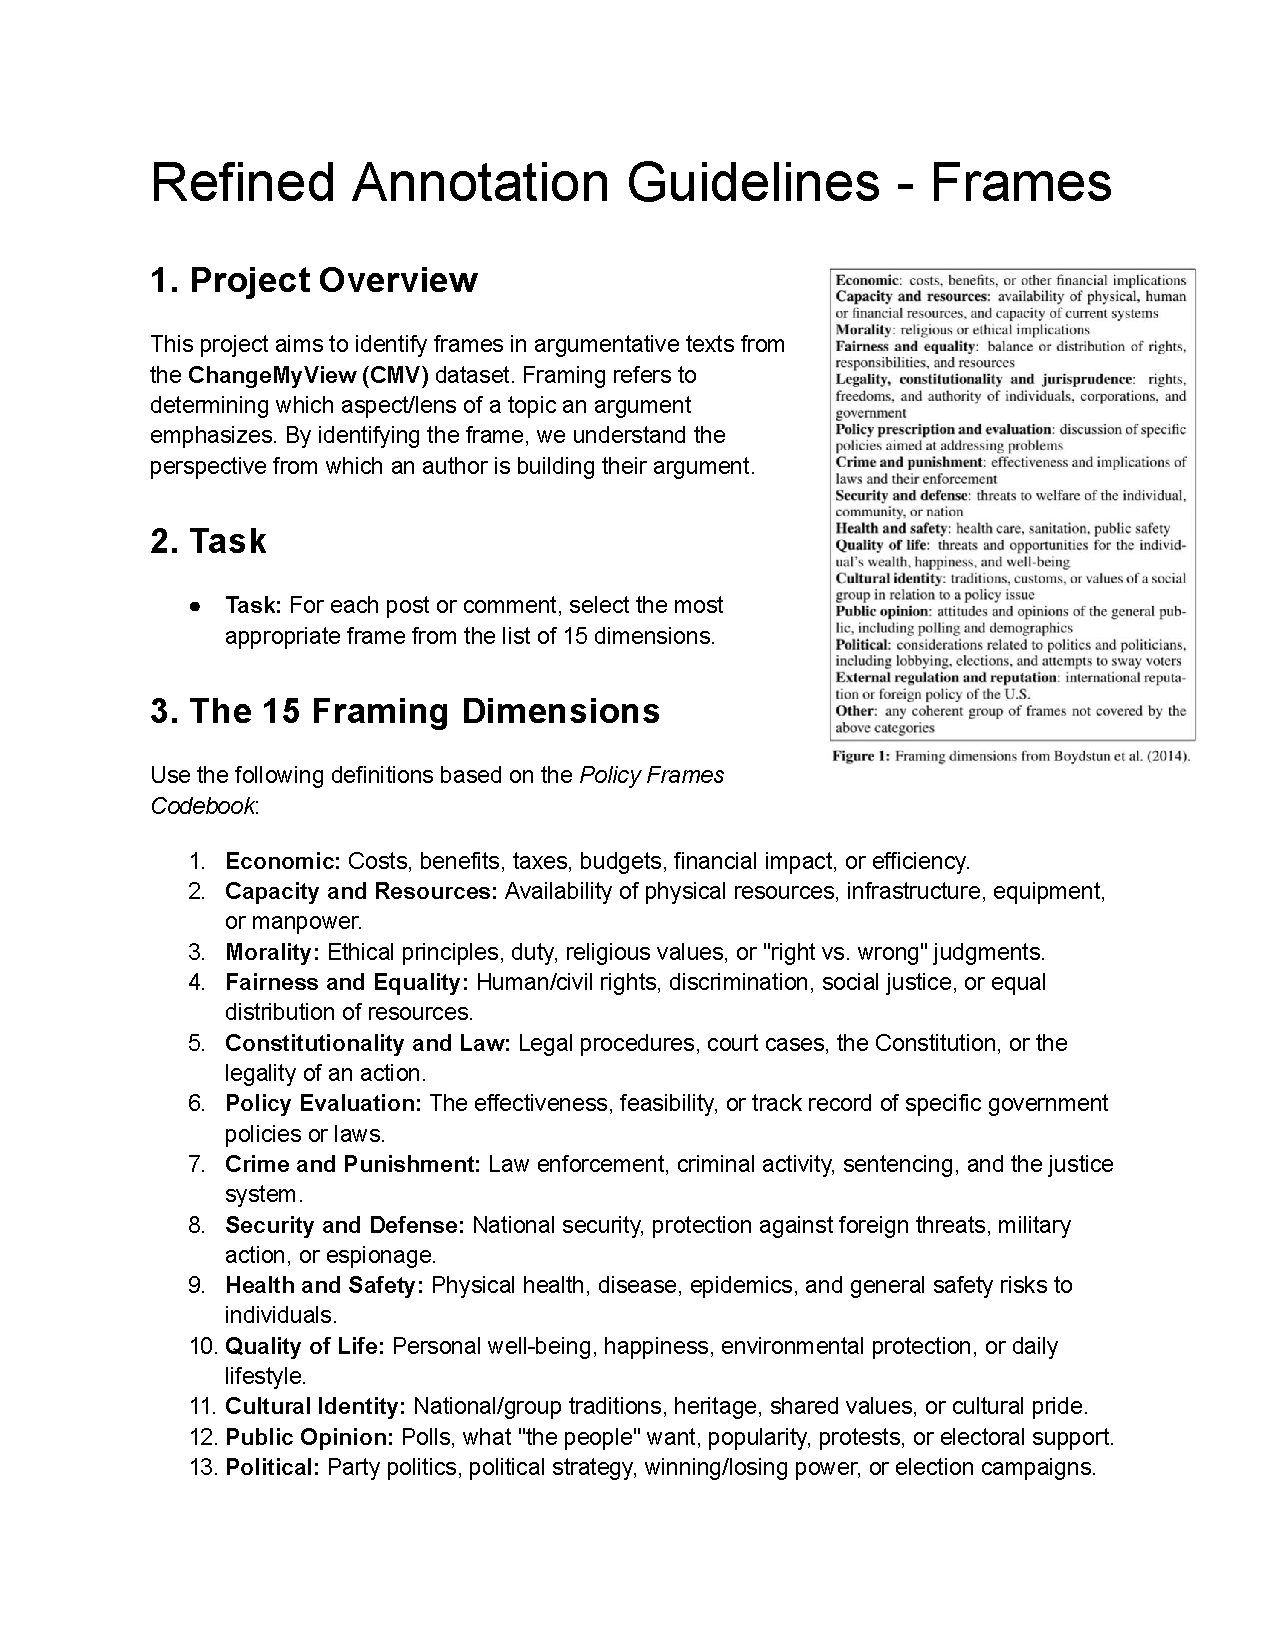
\includegraphics[page=1,width=0.9\textwidth]{annotation_guidelines.pdf}
\end{center}

\includepdf[pages=2-,width=0.9\textwidth]{annotation_guidelines.pdf}

\newpage

\section{Results per annotator pre-adjudication}
\begin{table}[htbp]
\centering
\begin{tabular}{|l|c|c|c|c|}
\hline
\textbf{Frame} & \textbf{Accuracy} & \textbf{Precision} & \textbf{Recall} & \textbf{f1} \\
\hline
Capacity and Resources & 0.965 & 0.8750 & 0.5385 & 0.6667 \\\hline
Crime and Punishment & 0.985 & 0.7500 & 0.8571 & 0.8000 \\\hline
Cultural Identity & 0.940 & 0.9556 & 0.8113 & 0.8776 \\\hline
Economic & 0.980 & 0.9286 & 0.9286 & 0.9286 \\\hline
External Regulation and Reputation & 0.985 & 0.5000 & 0.6667 & 0.5714 \\\hline
Fairness and Equality & 0.955 & 0.8293 & 0.9444 & 0.8831 \\\hline
Health and Safety & 0.980 & 0.8947 & 0.8947 & 0.8947 \\\hline
Legality, Constitutionality and Jurisprudence & 0.950 & 0.9091 & 0.7143 & 0.8000 \\\hline
Morality & 0.950 & 0.8571 & 0.9818 & 0.9153 \\\hline
Other & 0.960 & 0.7308 & 0.9500 & 0.8261 \\\hline
Policy Prescription and Evaluation & 0.950 & 0.7692 & 0.8333 & 0.8000 \\\hline
Political & 0.985 & 0.8929 & 1.0000 & 0.9434 \\\hline
Public Opinion & 0.945 & 0.7619 & 0.7273 & 0.7442 \\\hline
Quality of Life & 0.955 & 0.8485 & 0.8750 & 0.8615 \\\hline
Security and Defense & 0.995 & 0.8750 & 1.0000 & 0.9333 \\
\hline
\textbf{Total for all frames} & 0.725 & 0.8625 & 0.8879 & 0.8658 \\
\hline
\end{tabular}
\caption{Performance of Annotator 1 pre-adjudication.}
\label{tab:pre_annotator1_performance}
\end{table}

\begin{table}[htbp]
\centering
\begin{tabular}{|l|c|c|c|c|}
\hline
\textbf{Frame} & \textbf{Accuracy} & \textbf{Precision} & \textbf{Recall} & \textbf{f1} \\
\hline
Capacity and Resources & 0.965 & 0.6667 & 0.9231 & 0.7742 \\\hline
Crime and Punishment & 0.985 & 0.7000 & 1.0000 & 0.8235 \\\hline
Cultural Identity & 0.885 & 0.7419 & 0.8679 & 0.8000 \\\hline
Economic & 0.980 & 0.8750 & 1.0000 & 0.9333 \\\hline
External Regulation and Reputation & 0.985 & 0.5000 & 0.6667 & 0.5714 \\\hline
Fairness and Equality & 0.935 & 0.8485 & 0.7778 & 0.8116 \\\hline
Health and Safety & 0.940 & 0.6522 & 0.7895 & 0.7143 \\\hline
Legality, Constitutionality and Jurisprudence & 0.965 & 0.8387 & 0.9286 & 0.8814 \\\hline
Morality & 0.925 & 0.8571 & 0.8727 & 0.8649 \\\hline
Other & 0.975 & 1.0000 & 0.7500 & 0.8571 \\\hline
Policy Prescription and Evaluation & 0.945 & 0.8824 & 0.6250 & 0.7317 \\\hline
Political & 0.975 & 0.9545 & 0.8400 & 0.8936 \\\hline
Public Opinion & 0.965 & 0.7778 & 0.9545 & 0.8571 \\\hline
Quality of Life & 0.910 & 0.7917 & 0.5938 & 0.6786 \\\hline
Security and Defense & 0.970 & 0.5455 & 0.8571 & 0.6667 \\
\hline
\textbf{Total for all frames} & 0.560 & 0.8192 & 0.8408 & 0.8092 \\
\hline
\end{tabular}
\caption{Performance of Annotator 2 pre-adjudication.}
\label{tab:pre_annotator2_performance}
\end{table}

\begin{table}[htbp]
\centering
\begin{tabular}{|l|c|c|c|c|}
\hline
\textbf{Frame} & \textbf{Accuracy} & \textbf{Precision} & \textbf{Recall} & \textbf{f1} \\
\hline
Capacity and Resources & 0.945 & 0.5833 & 0.5385 & 0.5600 \\\hline
Crime and Punishment & 0.990 & 0.7778 & 1.0000 & 0.8750 \\\hline
Cultural Identity & 0.895 & 0.7581 & 0.8868 & 0.8174 \\\hline
Economic & 0.965 & 1.0000 & 0.7500 & 0.8571 \\\hline
External Regulation and Reputation & 0.985 & 0.5000 & 1.0000 & 0.6667 \\\hline
Fairness and Equality & 0.895 & 0.6667 & 0.8333 & 0.7407 \\\hline
Health and Safety & 0.970 & 0.8421 & 0.8421 & 0.8421 \\\hline
Legality, Constitutionality and Jurisprudence & 0.950 & 0.8462 & 0.7857 & 0.8148 \\\hline
Morality & 0.895 & 0.8696 & 0.7273 & 0.7921 \\\hline
Other & 0.930 & 0.6364 & 0.7000 & 0.6667 \\\hline
Policy Prescription and Evaluation & 0.905 & 0.5714 & 0.8333 & 0.6780 \\\hline
Political & 0.950 & 0.8947 & 0.6800 & 0.7727 \\\hline
Public Opinion & 0.910 & 0.5714 & 0.7273 & 0.6400 \\\hline
Quality of Life & 0.925 & 0.7429 & 0.8125 & 0.7761 \\\hline
Security and Defense & 0.985 & 1.0000 & 0.5714 & 0.7273 \\
\hline
\textbf{Total for all frames} & 0.520 & 0.7429 & 0.7796 & 0.7458 \\
\hline
\end{tabular}
\textbf{}\caption{Performance of Annotator 4 pre-adjudication.}
\label{tab:pre_annotator4_performance}
\end{table}

\newpage

\section{Duplicate comments}
\begin{table}[ht]
\centering
\renewcommand{\arraystretch}{1.25}

\begin{tabularx}{\textwidth}{|l|l|l|X|}
\hline
\textbf{ID} & \textbf{Task info} & \textbf{Annotator} & \textbf{Thread} \\ \hline

ch26fk7 & triple 20874 / single 21451 & 4 & CMV: I believe that current political campaign norms are wasteful \\ \hline

dcftrw0 & triple 20830 / single 21299 & 1 & CMV: I can't see why I should have to respect Christianity \\ \hline

deywptq & triple 20949 / single 21258 & 1 & CMV: The United States can and should act as the "World Police" \\ \hline

deyyihc & triple 20911 / single 21428 & 4 & Duplicate of #3: US as "World Police" \\ \hline

djeqp2j & triple 20862 / single 21222 & 1 & CMV: Personal problems do not justify being rude to others \\ \hline

\end{tabularx}

\caption{The duplicate comments found in the dataset.}
\label{tab:cmv_cleaning}

\end{table}

\newpage

\section{Results per annotator post-adjudication}

\begin{table}[htbp]
\small
\centering
\begin{tabular}{|l|c|c|c|c|}
\hline
\textbf{Frame} & \textbf{Accuracy} & \textbf{Precision} & \textbf{Recall} & \textbf{f1} \\
\hline
Capacity and Resources & 0.975 & 0.9000 & 0.6923 & 0.7826 \\\hline
Crime and Punishment & 0.985 & 0.7500 & 0.8571 & 0.8000 \\\hline
Cultural Identity & 0.940 & 0.9556 & 0.8113 & 0.8776 \\\hline
Economic & 0.980 & 0.9286 & 0.9286 & 0.9286 \\\hline
External Regulation and Reputation & 0.985 & 0.5000 & 0.6667 & 0.5714 \\\hline
Fairness and Equality & 0.960 & 0.8333 & 0.9722 & 0.8974 \\\hline
Health and Safety & 0.980 & 0.8947 & 0.8947 & 0.8947 \\\hline
Legality, Constitutionality and Jurisprudence & 0.950 & 0.9091 & 0.7143 & 0.8000 \\\hline
Morality & 0.950 & 0.8571 & 0.9818 & 0.9153 \\\hline
Other & 0.970 & 0.7917 & 0.9500 & 0.8636 \\\hline
Policy Prescription and Evaluation & 0.955 & 0.7778 & 0.8750 & 0.8235 \\\hline
Political & 0.985 & 0.8929 & 1.0000 & 0.9434 \\\hline
Public Opinion & 0.955 & 0.7826 & 0.8182 & 0.8000 \\\hline
Quality of Life & 0.960 & 0.8529 & 0.9062 & 0.8788 \\\hline
Security and Defense & 0.995 & 0.8750 & 1.0000 & 0.9333 \\
\hline
\textbf{Total for all frames} & 0.745 & 0.8725 & 0.9029 & 0.8791 \\
\hline
\end{tabular}
\caption{Performance of Annotator 1 post-adjudication.}
\label{tab:post_annotator1_performance}
\end{table}

\newpage

\begin{table}[htbp]
\small
\centering
\begin{tabular}{|l|c|c|c|c|}
\hline
\textbf{Frame} & \textbf{Accuracy} & \textbf{Precision} & \textbf{Recall} & \textbf{f1} \\
\hline
Capacity and Resources & 0.965 & 0.6667 & 0.9231 & 0.7742 \\\hline
Crime and Punishment & 0.985 & 0.7000 & 1.0000 & 0.8235 \\\hline
Cultural Identity & 0.890 & 0.7541 & 0.8679 & 0.8070 \\\hline
Economic & 0.980 & 0.8750 & 1.0000 & 0.9333 \\\hline
External Regulation and Reputation & 0.985 & 0.5000 & 0.6667 & 0.5714 \\\hline
Fairness and Equality & 0.940 & 0.8529 & 0.8056 & 0.8286 \\\hline
Health and Safety & 0.940 & 0.6522 & 0.7895 & 0.7143 \\\hline
Legality, Constitutionality and Jurisprudence & 0.965 & 0.8387 & 0.9286 & 0.8814 \\\hline
Morality & 0.930 & 0.8596 & 0.8909 & 0.8750 \\\hline
Other & 0.975 & 1.0000 & 0.7500 & 0.8571 \\\hline
Policy Prescription and Evaluation & 0.950 & 0.8889 & 0.6667 & 0.7619 \\\hline
Political & 0.980 & 0.9565 & 0.8800 & 0.9167 \\\hline
Public Opinion & 0.965 & 0.7778 & 0.9545 & 0.8571 \\\hline
Quality of Life & 0.920 & 0.8077 & 0.6562 & 0.7241 \\\hline
Security and Defense & 0.970 & 0.5455 & 0.8571 & 0.6667 \\
\hline
\textbf{Total for all frames} & 0.580 & 0.8217 & 0.8521 & 0.8181 \\
\hline
\end{tabular}
\caption{Performance of Annotator 2 post-adjudication.}
\label{tab:post_annotator2_performance}
\end{table}


\begin{table}[htbp]
\small
\centering
\begin{tabular}{|l|c|c|c|c|}
\hline
\textbf{Frame} & \textbf{Accuracy} & \textbf{Precision} & \textbf{Recall} & \textbf{f1} \\
\hline
Capacity and Resources & 0.955 & 0.6429 & 0.6923 & 0.6667 \\\hline
Crime and Punishment & 0.990 & 0.7778 & 1.0000 & 0.8750 \\\hline
Cultural Identity & 0.900 & 0.7705 & 0.8868 & 0.8246 \\\hline
Economic & 0.965 & 1.0000 & 0.7500 & 0.8571 \\\hline
External Regulation and Reputation & 0.985 & 0.5000 & 1.0000 & 0.6667 \\\hline
Fairness and Equality & 0.900 & 0.6818 & 0.8333 & 0.7500 \\\hline
Health and Safety & 0.970 & 0.8421 & 0.8421 & 0.8421 \\\hline
Legality, Constitutionality and Jurisprudence & 0.950 & 0.8462 & 0.7857 & 0.8148 \\\hline
Morality & 0.900 & 0.8723 & 0.7455 & 0.8039 \\\hline
Other & 0.935 & 0.6667 & 0.7000 & 0.6829 \\\hline
Policy Prescription and Evaluation & 0.910 & 0.5882 & 0.8333 & 0.6897 \\\hline
Political & 0.955 & 0.9000 & 0.7200 & 0.8000 \\\hline
Public Opinion & 0.920 & 0.6000 & 0.8182 & 0.6923 \\\hline
Quality of Life & 0.935 & 0.7568 & 0.8750 & 0.8116 \\\hline
Security and Defense & 0.985 & 1.0000 & 0.5714 & 0.7273 \\
\hline
\textbf{Total for all frames} & 0.540 & 0.7554 & 0.7958 & 0.7608 \\
\hline
\end{tabular}
\caption{Performance of Annotator 4 post-adjudication.}
\label{tab:post_annotator4_performance}
\end{table}



\section{Prompt Engineering}
\label{app:annotation-prompt}
\begin{tcolorbox}[
    colback=gray!5,
    colframe=black!75,
    title=Prompt Used for LLM Frame Annotation,
    sharp corners,
    boxrule=0.5pt
]

\small

You are an expert annotator for framing analysis in argumentative discourse, using the Boydstun et al. (2014) media frame taxonomy.

\vspace{0.5em}

You will be given:

\begin{itemize}
    \item The original post (OP) of an r/ChangeMyView thread --- context only.
    \item A single comment replying to the OP --- the target for annotation.
\end{itemize}

For the comment (not the OP), identify which frames are present from the taxonomy below.

\vspace{0.5em}

\textbf{Frame Definitions}

\begin{itemize}
    \item \textbf{Economic}: Costs, benefits, or other financial implications.
    \item \textbf{Capacity and Resources}: Availability of physical, human, or financial resources, and system capacity.
    \item \textbf{Morality}: Religious or ethical implications.
    \item \textbf{Fairness and Equality}: Distribution of rights, responsibilities, and resources.
    \item \textbf{Legality, Constitutionality and Jurisprudence}: Rights, freedoms, and authority of individuals, corporations, and government, including constitutional or legal interpretation.
    \item \textbf{Policy Prescription and Evaluation}: Discussion of specific policies aimed at addressing or evaluating problems.
    \item \textbf{Crime and Punishment}: Effectiveness, fairness, and implications of laws and their enforcement.
    \item \textbf{Security and Defense}: Threats to the safety of individuals, communities, or nations.
    \item \textbf{Health and Safety}: Issues related to healthcare, sanitation, and public safety.
    \item \textbf{Quality of Life}: Impacts on individual wealth, happiness, well-being, or life satisfaction.
    \item \textbf{Cultural Identity}: Traditions, customs, or values of social groups in relation to the issue.
    \item \textbf{Public Opinion}: Attitudes, beliefs, or polling of the general public.
    \item \textbf{Political}: Political actors, elections, lobbying, or strategic political considerations.
    \item \textbf{External Regulation and Reputation}: International relations, foreign policy, or global reputation.
    \item \textbf{Other}: Any coherent framing not captured by the above categories.
\end{itemize}

\vspace{0.5em}

\textbf{Rules}

\begin{itemize}
    \item A comment may include multiple frames (multi-label classification is allowed).
    \item Only assign a frame if it is substantively present, not if it is merely mentioned.
    \item Return JSON with exactly one key: \texttt{"comment\_frames"}.
    \item The value must be a list of frame labels using the exact names provided above.
    \item If no frames apply, return an empty list.
\end{itemize}

\vspace{0.5em}

\textbf{Input}

\textbf{Title:} \texttt{\{thread\_title\}}

\textbf{Original Post (context only):}

\texttt{\{thread\_body\}}

\textbf{Comment to annotate:}

\texttt{\{comment\_body\}}

\end{tcolorbox}

\section{Annotation guideline questionnaire}
\label{sec:guidelines_questionnaire}

 Please read each comment carefully and determine which "frame" the author is using to make their point.  \\

\textbf{Rules}

\begin{itemize}
\item Select 1 or 2 frames: If an argument clearly touches on two perspectives, please select both.

\item However, when choosing 'other', only 1 label is allowed

\item Be Critical: In part two you will see suggestions provided by an AI. Please use your own judgment to decide if the AI is correct or if a different frame fits better.

\end{itemize}

\textbf{Examples}

\begin{itemize}
\item ``CMV: Religion has no positive attributes.'' \
$\rightarrow$ \textit{Morality}

\item ``CMV: Most `big words' have no place outside of formal writing or speeches.'' \\
$\rightarrow$ \textit{Other}

\item ``CMV: Money to me is a renewable source so I just spend it knowing I'll get paid again so it'll come back.'' \\
$\rightarrow$ \textit{Economic}

\item ``CMV: There are no adequate gender-equal options when it comes to changing your surname in marriage.'' \\
$\rightarrow$ \textit{Fairness and Equality}

\item ``CMV: I believe that blacks are genetically inferior to whites, Asians, and Jews as far as intelligence is concerned.'' \\
$\rightarrow$ This could either be \textit{Morality} or \textit{Cultural Identity} , so both labels can be chosen.


\end{itemize}


\textbf{The frames:}\\

You will choose from the 15 frames defined \cite{card2015media}, see (the table) below. The frames and a brief description of each frame will be provided with every question to help you choose.


\begin{itemize}
    \item \textbf{Economic} — Costs, benefits, or other financial implications.

    \item \textbf{Capacity and Resources} — Availability of physical, human, or financial resources, and capacity of current systems.

    \item \textbf{Morality} — Religious or ethical implications.

    \item \textbf{Fairness and Equality} — Balance or distribution of rights, responsibilities, and resources.

    \item \textbf{Legality, Constitutionality and Jurisprudence} — Rights, freedoms, and authority of individuals, corporations, and government.

    \item \textbf{Policy Prescription and Evaluation} — Discussion of specific policies aimed at addressing problems.

    \item \textbf{Crime and Punishment} — Effectiveness and implications of laws and their enforcement.

    \item \textbf{Security and Defense} — Threats to the welfare of the individual, community, or nation.

    \item \textbf{Health and Safety} — Health care, sanitation, and public safety.

    \item \textbf{Quality of Life} — Threats and opportunities for an individual's wealth, happiness, and well-being.

    \item \textbf{Cultural Identity} — Traditions, customs, or values of a social group in relation to a policy issue.

    \item \textbf{Public Opinion} — Attitudes and opinions of the general public, including polling and demographics.

    \item \textbf{Political} — Considerations related to politics and politicians, including lobbying, elections, and attempts to sway voters.

    \item \textbf{External Regulation and Reputation} — International reputation or foreign policy of the United States.

    \item \textbf{Other} — Any coherent group of frames not covered by the above categories.
\end{itemize}


\section{Questionnaire}
\footnotesize
\renewcommand{\arraystretch}{1.15}

\begin{longtable}{|c|p{4cm}|p{8cm}|}
\caption{Comments and gold frames of Part A of the forms.}
\label{tab:questionnaire} \\

\hline
\textbf{\#} & \textbf{Gold Frames} & \textbf{Comment} \\ \hline
\endfirsthead

\hline
\textbf{\#} & \textbf{Gold Frames} & \textbf{Comment} \\ \hline
\endhead

1 & morality + fairness and equality & Children deserve no respect because they cant hurt you. Once they are big enough, you can respect them \\ \hline

2 & cultural identity & I would mind and FEAR if they acted like us on THEIR OWN. \\ \hline

3 & external regulation and reputation & It's a geographical thing -- westerners have no right to organize protests on the domestic policies of the easterners, just as easterners have no right to criticize the west for its domestic policies. \\ \hline

4 & fairness and equality + crime and punishment & Aren't public officials the only people that CAN engage in corruption? How do you make all corruption sentences stronger than the average corruption sentence? \\ \hline

5 & morality + public opinion & If people can realize they're OK with some GMOs outside the food chain, they might think differently about the GMOs they are against inside the food chain. \\ \hline

6 & morality + cultural identity & I don't know if it matters to you at all (I bring it up because many politicians claim Christianity), but the Bible pretty much teaches what you're saying. Those in leadership positions should be held to a higher standard and be beyond reproach. \\ \hline

7 & capacity and resources & In many countries any commercial content in schools is forbidden (e.g. Israel). \\ \hline

8 & other & When that person shoots you because no one cared about or understood his problems/frustration, maybe that will change your mind. \\ \hline

9 & political + public opinion & The fact that Hillary stole the primary from Bernie left a lot of rightfully salty Bernie supporters. Many stuck with Clinton for the general, some wrote in Bernie, some probably didn't vote, some went third, and some probably went over to Trump, would you believe. \\ \hline

10 & policy prescription and evaluation & Civil forfeiture has done some good. Forfeiture programs ``have crippled powerful drug-trafficking organizations''. \\ \hline

11 & quality of life + cultural identity & Naturally letting society evolve to tolerate differences will almost undoubtedly lead to a higher tolerance of those differences than having the state enforce tolerance. \\ \hline

12 & other & The GOP has no choice. The roles forgot the PSU from kicking the nominee out at this point. QED. \\ \hline

13 & quality of life + capacity and resources & I think the most realistic outcome of the development of strong AI is not a black and white scenario where there are the big scary evil ``Robots'' and the weakened soft fleshy ``Humans'' are forever separate; instead, surely we'll slowly merge with robots / robots will slowly merge with us. \\ \hline

14 & economic + fairness and equality & An important thing to realize is that these issues come from the economic system. Let's look at capitalism and sexism. When sexism is taught and shown all around us, it is much easier to pay women less than men, increasing profit. Then when they are stay-at-home baby makers, they can produce workers and make sure they can work in 20 years and be better with mommy's 100\% attention. Sexism is profitable. \\ \hline

15 & quality of life + public opinion & Why would a larger audience for this deception make the world a better place and not a more confused place? \\ \hline

16 & morality & To some people, the base meaning of respect is to be treated like a person. To others, the base meaning of respect is to be treated like an authority. \\ \hline

17 & crime and punishment + public opinion & You would advocate the use of force to stop someone from tipping? That is to say, you would put someone in jail if they tipped someone else? What about the person who accepts that tip? Is he an accomplice to the crime? \\ \hline

18 & economic & Children seem like a horribly inefficient retirement plan. If you are only concerned about the financial aspects, it would be way cheaper to take the money you would have spent raising children, put it in an IRA invested in an index fund, and you'll come out in pretty good shape financially when retirement rolls around. \\ \hline

19 & health and safety + policy prescription & It says non-FDA-approved drugs; it specifically mentions that they should be currently undergoing trials. \\ \hline

20 & morality & Now let's imagine it's ``human'' -- like us, as you say. It would feel power, greed, etc., the nasty stuff. But it would also feel empathy, and in fact that is what an AI needs to not become evil. \\ \hline

\end{longtable}

\small
\renewcommand{\arraystretch}{1.2}

\begin{longtable}{|c|p{2.5cm}|p{2.5cm}|p{2.5cm}|p{4.0cm}|}
\caption{Comments, gold frames, LLM suggestions of Part B of the forms.}
\label{tab:llm_predictions} \\

\hline
\textbf{\#} & \textbf{Right Frames} & \textbf{LLM Suggestion} & \textbf{Correct/incorrect suggestion}  & \textbf{Comment} \\ \hline
\endfirsthead

\hline
\textbf{\#} & \textbf{Gold Frames} & \textbf{LLM Suggestion} & \textbf{Correct/incorrect suggestion} & \textbf{Comment} \\ \hline
\endhead

21 & quality of life & quality of life & correct & You really think out of billions of people there aren't people who enjoy and build a strong relationship out of the game of ``winning one another over'' though? \\ \hline

22 & morality + public opinion & economic & incorrect & No you're wrong. If the media gave us the facts and told the truth instead of throwing their worthless opinions in we could watch more reliable television. \\ \hline

23 & other & other & correct & Being still and alert for hours at a time, that upper level eSport participants do, is a physical exertion. It's physical because it requires sitting in one spot and being alert. It's an exertion because you are sore and tired at the end of it. \\ \hline

24 & morality & external regulation & incorrect & He's your answer: respect everyone unless proven otherwise. \\ \hline

25 & Legality, constitutionality and jurisprudence + morality & Legality, constitutionality and jurisprudence + morality & correct & What if the only way to ``legally'' obtain a movie is to pay \$1,000,000 dollars for it? Would it be immoral to pirate that? \\ \hline

26 & economic + fairness and equality & capacity and resources & incorrect & Gender inequality \textbf{is} a huge economic issue for half the population who are underpaid for their work or discriminated against for promotion etc. \\ \hline

27 & economic + quality of life & economic + quality of life & correct & Every child is a retirement plan. I hope I raise my kids to make a better world. A world that will make my elderly ass easier. \\ \hline

28 & fairness and equality & fairness and equality & correct & Do you see the problem here? It is intentionally obtuse to argue that diversity is unrelated to discrimination. Problems with discrimination are what give rise to the appeal of diversity in the first place. \\ \hline

29 & crime and punishment & public opinion & incorrect & As for reason 1, I would argue that death, even at your own choosing, is the ultimate punishment. \\ \hline

30 & Legality, constitutionality and jurisprudence + fairness and equality & Legality, constitutionality and jurisprudence + fairness and equality & correct & Sites stealing Reddit content?! Reddit content is stolen off other sites too -- not to mention 99\% of images are posted to Imgur, lacking any attribution to the original creator, much less the site they were taken from. \\ \hline

31 & security and defense + morality & security and defense + morality & correct & What I've said is precisely what I'm saying: that if gay pride parades are part of a strategy to improve gay rights, they are, at this time, doing more harm than good. \\ \hline

32 & external regulation and reputation & health and safety & incorrect & The United States, being the only nation on earth that currently has the military capacity to destroy any other regime on earth, has a duty and a responsibility to function as a de-facto police force for the world. \\ \hline

33 & economic + crime and punishment & health and safety + policy prescription & correct & Why should it be illegal to give someone a small sum of money for good service? Who are you to tell an entire nation that practice is not to be allowed? \\ \hline

34 & morality & political & incorrect & Yeah, and my contention is that your view is not only different than mine, but morally wrong. \\ \hline

35 & economic & economic & correct & Advertisements should be allowed in school because it is an easy way to generate revenue and as you noted there would be high demand to advertise in schools since kids are such an important demographic for marketers. \\ \hline

36 & economic + policy prescription and evaluation & morality & incorrect & I believe that you are missing an enormous part of campaigning with your proposed reforms, namely the \textit{soft money} campaigning of corporations, unions, and the more wealthy members of the US. \\ \hline

37 & Legality, constitutionality and jurisprudence + policy evaluation & Legality, constitutionality and jurisprudence + policy evaluation & correct & That being said, expanding that judgment to people with clean records and a single traffic violation in question is clearly a case of a poorly written rule set. \\ \hline

38 & fairness and equality + quality of life & security and defense & incorrect & I have spoken to Glaswegians, Californians, Texans, Aussies, Kiwis, Corkmen, Dubliners etc. and they've \textit{all} spoken the same language. Sometimes they have slight differences in word preference, and they often have different slang. They always have significant differences in pronunciation. \\ \hline

39 & Legality, constitutionality and jurisprudence & capacity and resources & incorrect & When you steal, you don't gain ownership of whatever you stole, you merely have it in your possession. The person from whom it was stolen still has ownership. \\ \hline

40 & other & public opinion & incorrect & Even Reuters and AP are inherently editorialized through omission, selection, language, geography, and so forth. You can't really have ``Just the facts'' unless you have all the facts. \\ \hline

\end{longtable}

\newpage

\section{Mean of results per annotator (pre- and post-adjudication}
\begin{table}[htbp]
\centering
\small
\begin{tabular}{|l|c|c|c|c|}
\hline
\textbf{Frame} & \textbf{Accuracy} & \textbf{Precision} & \textbf{Recall} & \textbf{f1} \\
\hline
Capacity and Resources & 0.9583 & 0.7083 & 0.6667 & 0.6670 \\\hline
Crime and Punishment & 0.9867 & 0.7426 & 0.9524 & 0.8328 \\\hline
Cultural Identity & 0.9067 & 0.8185 & 0.8553 & 0.8317 \\\hline
Economic & 0.9750 & 0.9345 & 0.8929 & 0.9063 \\\hline
External Regulation and Reputation & 0.9850 & 0.5000 & 0.7778 & 0.6032 \\\hline
Fairness and Equality & 0.9283 & 0.7815 & 0.8518 & 0.8118 \\\hline
Health and Safety & 0.9633 & 0.7963 & 0.8421 & 0.8170 \\\hline
Legality, Constitutionality and Jurisprudence & 0.9550 & 0.8647 & 0.8095 & 0.8321 \\\hline
Morality & 0.9233 & 0.8613 & 0.8606 & 0.8574 \\\hline
Other & 0.9550 & 0.7891 & 0.8000 & 0.7833 \\\hline
Policy Prescription and Evaluation & 0.9333 & 0.7410 & 0.7639 & 0.7366 \\\hline
Political & 0.9700 & 0.9140 & 0.8400 & 0.8699 \\\hline
Public Opinion & 0.9400 & 0.7037 & 0.8030 & 0.7471 \\\hline
Quality of Life & 0.9300 & 0.7944 & 0.7604 & 0.7721 \\\hline
Security and Defense & 0.9833 & 0.8068 & 0.8095 & 0.7758 \\\hline
TOTAL (Mean of Annotators) & 0.6017 & 0.8082 & 0.8361 & 0.8069 \\
\hline
\end{tabular}
\caption{Mean performance across annotators by frame (pre-adjudication).}
\label{tab:pre-mean_annotator_performance}
\end{table}

\begin{table}[htbp]
\centering
\small
\begin{tabular}{|l|c|c|c|c|}
\hline
\textbf{Frame} & \textbf{Accuracy} & \textbf{Precision} & \textbf{Recall} & \textbf{f1} \\
\hline
Capacity and Resources & 0.9650 & 0.7365 & 0.7692 & 0.7412 \\\hline
Crime and Punishment & 0.9867 & 0.7426 & 0.9524 & 0.8328 \\\hline
Cultural Identity & 0.9100 & 0.8267 & 0.8553 & 0.8364 \\\hline
Economic & 0.9750 & 0.9345 & 0.8929 & 0.9063 \\\hline
External Regulation and Reputation & 0.9850 & 0.5000 & 0.7778 & 0.6032 \\\hline
Fairness and Equality & 0.9333 & 0.7893 & 0.8704 & 0.8253 \\\hline
Health and Safety & 0.9633 & 0.7963 & 0.8421 & 0.8170 \\\hline
Legality, Constitutionality and Jurisprudence & 0.9550 & 0.8647 & 0.8095 & 0.8321 \\\hline
Morality & 0.9267 & 0.8630 & 0.8727 & 0.8647 \\\hline
Other & 0.9600 & 0.8195 & 0.8000 & 0.8012 \\\hline
Policy Prescription and Evaluation & 0.9383 & 0.7516 & 0.7917 & 0.7584 \\\hline
Political & 0.9733 & 0.9165 & 0.8667 & 0.8867 \\\hline
Public Opinion & 0.9467 & 0.7201 & 0.8636 & 0.7831 \\\hline
Quality of Life & 0.9383 & 0.8058 & 0.8125 & 0.8048 \\\hline
Security and Defense & 0.9833 & 0.8068 & 0.8095 & 0.7758 \\\hline
TOTAL (Mean of Annotators) & 0.6217 & 0.8165 & 0.8503 & 0.8193 \\
\hline
\end{tabular}
\caption{Mean performance across annotators by frame (post-adjudication).}
\label{tab:post_mean_annotator_performance}
\end{table}

\newpage

\section{Per-frame F1 scores across groups}
\begin{table}[htbp]
\centering
\scriptsize
\setlength{\tabcolsep}{4pt}
\begin{tabular}{lccc}
\toprule
\textbf{Category} & \textbf{Overall} & \textbf{Part A} & \textbf{Part B} \\
\midrule

\multicolumn{4}{l}{\textbf{Group A}} \\
economic & 0.6667 & 0.7895 & 0.6053 \\
capacity/resources & 0.0000 & 0.0000 & 0.0000 \\
morality & 0.5285 & 0.4632 & 0.5918 \\
fairness/equality & 0.5210 & 0.4231 & 0.5970 \\
law/constitution & 0.6022 & 0.0000 & 0.7568 \\
policy eval & 0.1370 & 0.1081 & 0.1667 \\
crime/punishment & 0.2647 & 0.2927 & 0.2222 \\
security/defense & 0.0000 & 0.0000 & 0.0000 \\
health/safety & 0.1290 & 0.1667 & 0.0000 \\
quality of life & 0.4950 & 0.2800 & 0.7059 \\
cultural identity & 0.2222 & 0.2593 & 0.0000 \\
public opinion & 0.2174 & 0.3175 & 0.0000 \\
political & 0.4865 & 0.5455 & 0.0000 \\
external reg. & 0.2353 & 0.1250 & 0.3333 \\
other & 0.1818 & 0.1176 & 0.2373 \\
\midrule

\multicolumn{4}{l}{\textbf{Group B}} \\
economic & 0.6306 & 0.8718 & 0.5000 \\
capacity/resources & 0.1364 & 0.2222 & 0.0000 \\
morality & 0.5340 & 0.5287 & 0.5385 \\
fairness/equality & 0.3385 & 0.2182 & 0.4267 \\
law/constitution & 0.5155 & 0.0000 & 0.6579 \\
policy eval & 0.3678 & 0.3721 & 0.3636 \\
crime/punishment & 0.3492 & 0.5556 & 0.0741 \\
security/defense & 0.0741 & 0.0000 & 0.1053 \\
health/safety & 0.3243 & 0.3750 & 0.0000 \\
quality of life & 0.4854 & 0.3922 & 0.5769 \\
cultural identity & 0.2326 & 0.3125 & 0.0000 \\
public opinion & 0.1875 & 0.2373 & 0.1081 \\
political & 0.3404 & 0.4706 & 0.0000 \\
external reg. & 0.3871 & 0.3333 & 0.4211 \\
other & 0.2931 & 0.2759 & 0.3103 \\
\bottomrule
\end{tabular}
\caption{Per-frame F1 scores across conditions with and without LLM suggestions, split by task order.}
\label{tab:per_frame_f1_study}
\end{table}


\end{document}
